%% Dokumentklasse KOMA-Script Report
\documentclass[paper=a4, 12pt]{scrreprt}
%% Encoding UTF8
\usepackage[utf8]{inputenc}
%% 8 Bit Aufloesung der Buchstaben
\usepackage[T1]{fontenc}
%% Seitenraender
\usepackage[scale=0.72]{geometry}
%% Spracheinstellungen
\usepackage[english, naustrian]{babel} % your native language must be the last one!!
%% erweiterte Farbenpalette
\usepackage[dvipsnames]{xcolor}
%% Abbildungen
\usepackage{graphicx}
%% Tabellen (erweitert)
\usepackage{tabularx}
%% TikZ + Circuit-TikZ (fuer Schaltungen)
\usepackage[europeanresistors, europeaninductors]{circuitikz}
%% Nuetzliche TikZ Libraries
\usetikzlibrary{arrows, automata, positioning}
%% mathematik
\usepackage{amsmath, amssymb}
%\usepackage{mathtools}	
%% pdf-einbindung
\usepackage{pdfpages}
%% scource-code einbindung
\usepackage{listings, scrhack} %scrhack vermeidet Umschaltung auf KOMA Floats..
\usepackage{courier}
%% euro-symbol
\usepackage{eurosym}
%% landcsape-seiten ermöglichen
\usepackage{lscape}

%% Diplomarbeits-Format
\usepackage{srdpdipa}

%% Abkuerzungsverzeichnis
\usepackage[]{acronym}

%% Todos
\usepackage[]{todonotes}

%% Ganttdiagramme
\usepackage{pgfgantt}

%% Subfigures
\usepackage[lofdepth]{subfig}

%% Quotes
\usepackage{csquotes}

%%Comments
\usepackage{comment}
\excludecomment{comment}

%% definitionen =====================================%%
\dataSchool{HTBLuVA St. Pölten}
\dataDepartment{Höhere Lehranstalt für Elektronik und Technische Informatik}
\dataSubdepartment{Ausbildungsschwerpunkte Embedded- \& Wireless Systems}
\dataSession{2016/17}

\title{Bluetooth-Aktivbox}
\author{Markus Bointner \and Andreas Macsek}
\date{\today}
\place{St. P\"olten}
\professor{Prof. Dipl.-Ing. Dr. Herbert Wagner}
%%====================================================%%

% Hyperlinks im Dokument
\usepackage[colorlinks=true,
    linkcolor=black,
    citecolor=green,
    bookmarks=true,
    urlcolor=black,
    bookmarksopen=true]{hyperref}

\begin{document}

\frontmatter

%% titelseite ==========================================%%
\maketitle
%%======================================================%%

%% komplett leere seite ================================%%
\newpage\null\thispagestyle{empty}\newpage
%%======================================================%%

%% eidesstattliche erklärung ===========================%%
\begin{affidavit}
    \unterschrift{Markus Bointner}
    \unterschrift{Andreas Macsek}
\end{affidavit}
%%======================================================%%

%% dokumentation (deutsch/englisch) ====================%%
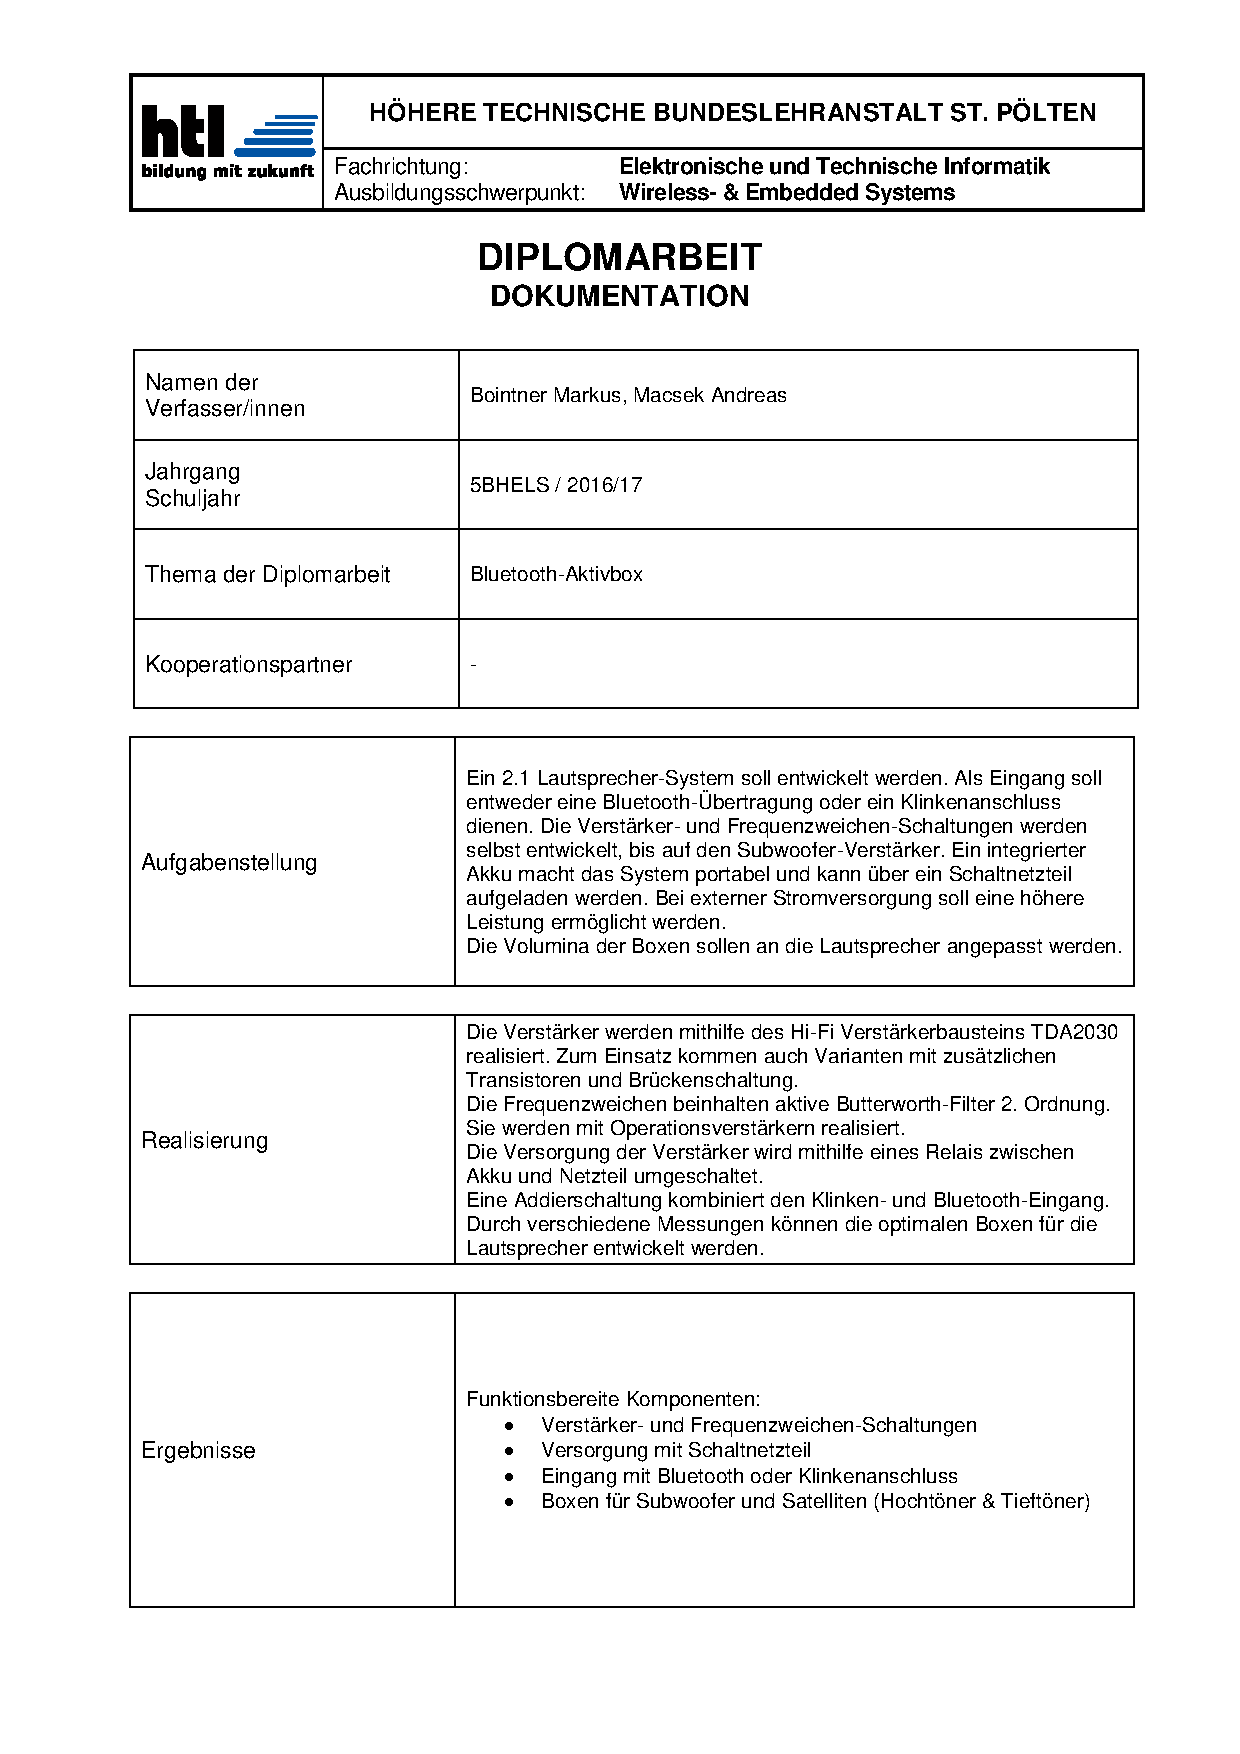
\includepdf[pages=-]{form/dokumentation-de.pdf}
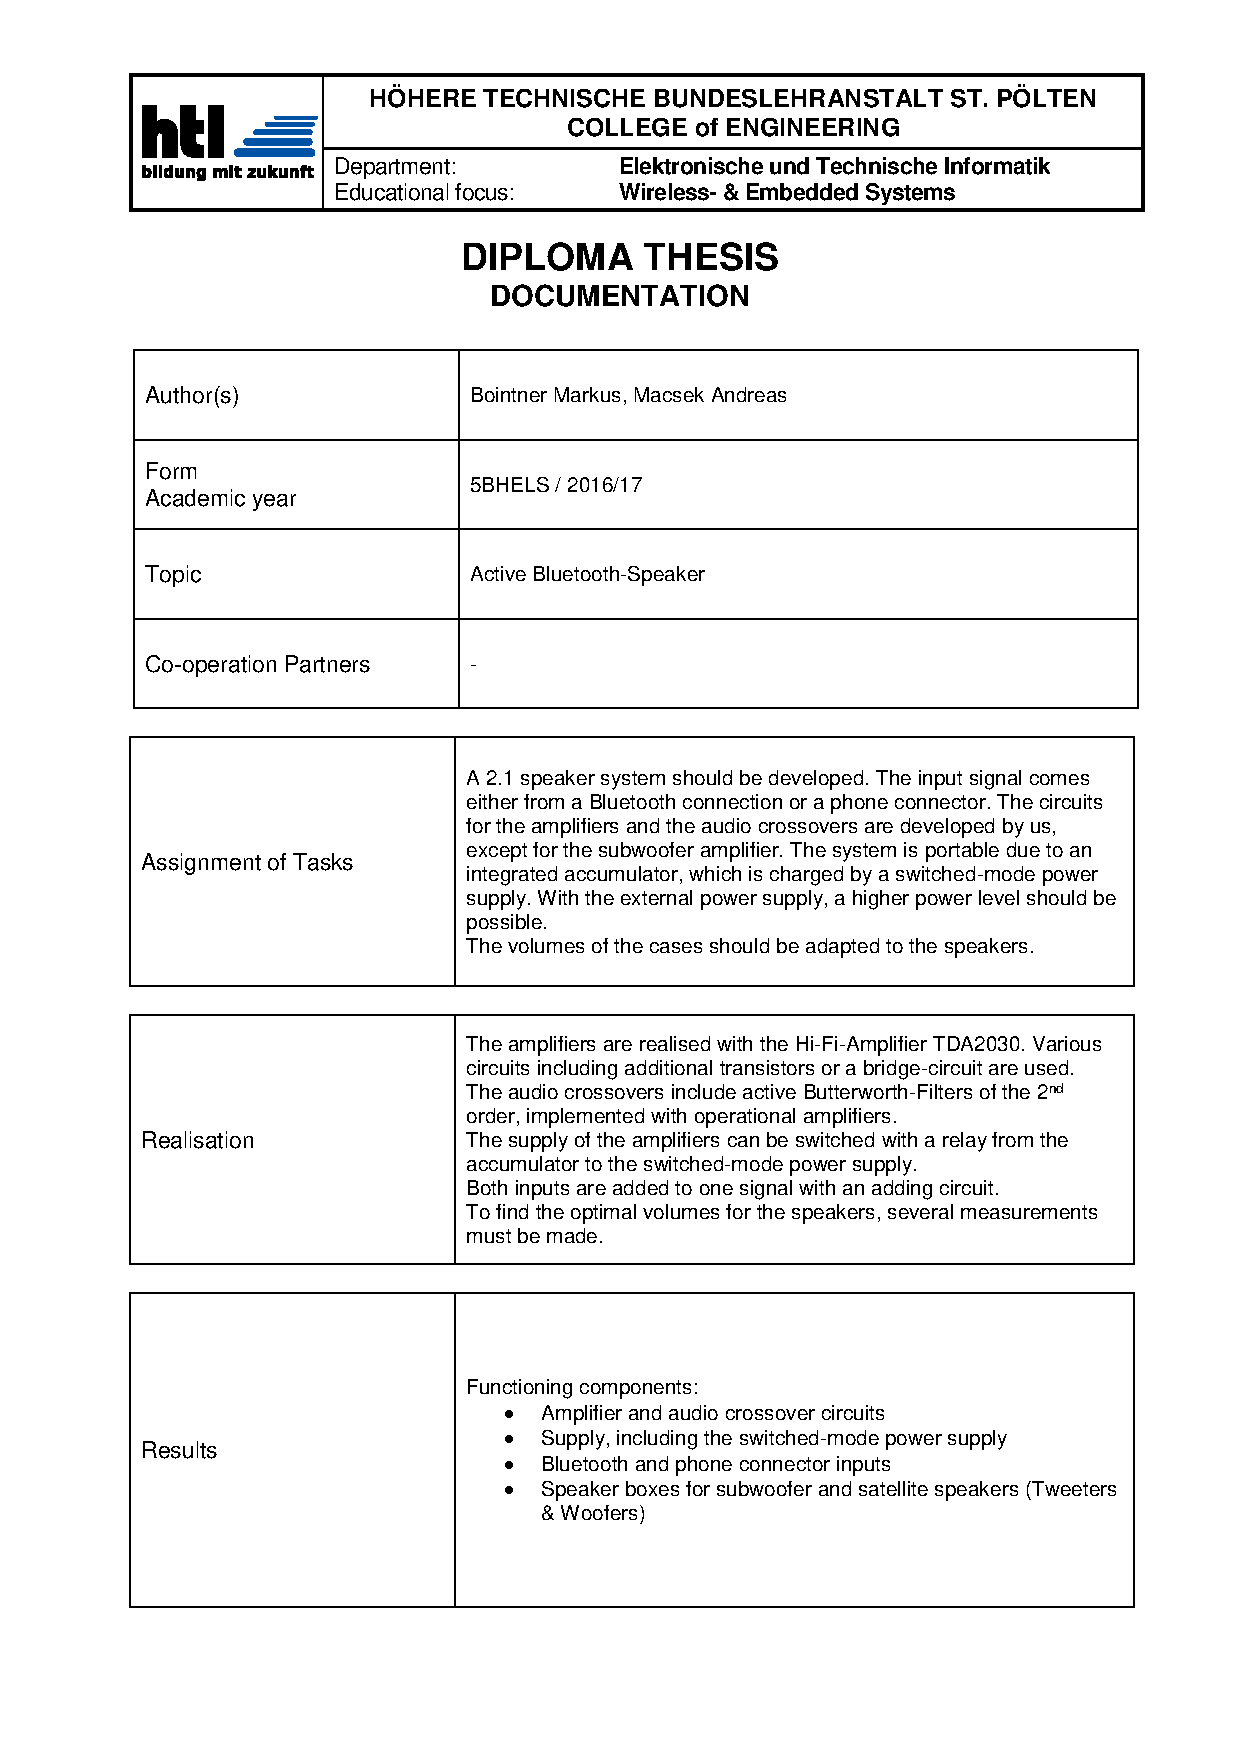
\includepdf[pages=-]{form/dokumentation-en.pdf}
%%======================================================%%

%% inhaltsverzeichnis ==================================%%
\tableofcontents
%%======================================================%%

%% HAUPTTEIL ===========================================%%
\responsible{Markus Bointner, Andreas Macsek}
\mainmatter

% Allgemeines über die Diplomarbeit
\chapter{Einleitung}
\responsible{Markus Bointner}
In diesem Kapitel wird erläutert, wie die Idee für diese Diplomarbeit entstanden ist und warum sie auch so verwirklicht wurde.

\section{Erste Idee} \label{sec:1.1}
Das Grundkonzept stammt von uns, also Markus Bointner und Andreas Macsek. Da wir beide von Musik begeistert sind, war es eine sehr interessante Idee für uns, selbst ein Lautsprechersystem zu entwickeln. Gleich zu Beginn war klar, dass wir noch ein kleines Extra mit einbauen wollten: eine Bluetooth-Ansteuerung.

\section{Weiterführende Gedanken} \label{sec:1.2}
Um all unsere Ideen zu verwirklichen, haben wir entschieden, diese Diplomarbeit ohne Firma und für den privaten Gebrauch zu entwickeln. Genauer gesagt ist das Lautsprechersystem dafür gedacht, im Freien oder in größeren Räumen Musik für kleinere Menschenmengen bereitzustellen. Das soll auch ohne externe Stromzufuhr funktionieren. Aus diesem Grund entstand dann die Idee einen Akku zu verbauen. Die manuelle Bedienung am Gerät soll mittels Ansteuerung eines Bluetooth-Moduls ermöglicht werden.


% Ziel der Diplomarbeit
\chapter{Gesamtprojekt}
\begin{comment}
\section{Ziele}\label{sec:2.1}
Es soll ein 2.1-System entwickelt werden.
Ein Mono-Subwoofer übernimmt den niedrigen Audiofrequenzbereich, während 2 weitere Lautsprecherboxen (auch genannt Satelliten-Boxen) - mit jeweils einem Hochton- und Tiefton-Lautsprecher - den Rest übernehmen.
Dieser Aufbau wurde gewählt um einen Raum-Klang erzeugen zu können. \\
Die Versorgung der Elektronik erfolgt entweder über Akku- oder Netzbetrieb.
Jeder Hochton- und Tiefton-Lautsprecher bekommt einen eigenen Verstärker (so auch der Mono-Subwoofer). \\
Das Audiosignal wird in verschiedene Frequenzbereiche aufgeteilt.\\

%An Struktur neu anpassen
Unsere Diplomarbeit kann grob in 2 Teile aufgeteilt werden:
\begin{itemize}
	\item Entwicklung der Elektronik
	\item Auswahl und Messungen der Lautsprecher
\end{itemize}
Die Ziele der 2 Teile werden in diesem Kapitel kurz erläutert.
\end{comment}

\subsection{Elektronik}\label{subsec:2.1.1}
Wie bereits in der Einleitung (\ref{sec:1.2}) erwähnt, ist das Projekt auch für den Akkubetrieb ausgelegt und benötigt daher eine passende Versorgungsschaltung.
Das Versorgungskonzept sieht einen 12V-Akku mit entsprechendem Ladegerät vor.
Dieses wurde zugekauft, da unser Projekt sich auf die Lautsprechermessung und -beschaltung konzentriert.
Bei Anschluss an eine Steckdose (nach CEE-Norm) übernimmt das vorgesehene Netzteil die Versorgung der Elektronik.
Wegen einer höheren Versorgungsspannung als die 12V des vorgesehenen Akkus, steht bei Netzbetrieb eine höhere Leistung zur Verfügung. \\ \\
Es werden analoge Verstärker verwendet.
Gründe dafür sind:
\begin{itemize}
	\item Einfacher Aufbau
	\item Ausreichende Leistung und Effizienz für dieses Projekt
	\item Bewährte Technik für Audioverstärker
\end{itemize} 
Das Audio-Signal muss vor den Verstärkern noch gefiltert werden.
Diese Aufgabe übernimmt eine Aktive Frequenzweiche.
Für den Mono-Subwoofer wird eine eigene Schaltung entwickelt die nicht nur die unerwünschten Signal-Anteile herausfiltert, sondern auch noch das Stereo-Signal auf ein Mono-Signal addiert.\\ \\
%\newpage ??
Die Signalaufnahme erfolgt über Eingänge auf der Hauptplatine.
Auf dieser Platine befindet sich ein AUX-Eingang (3,5mm Klinkenbuchse).
Über ein passendes Kinkensteckerkabel kann das Signal von einem beliebigen Endgerät wiedergegeben werden.
Eine weitere Möglichkeit bietet das Bluetooth-Modul, welches sich ebenfalls, mittels Adapterplatine, auf der Hauptplatine befindet.
Durch dieses kann über Bluetooth-Funkverbindung mit einem beliebigen bluetoothfähigen Endgerät ebenso ein Audiosignal übertragen werden.
An der Hauptplatine werden des weiteren Filter und an diesen die Verstärker angeschlossen. 
Das schlussendlich verstärkte und gefilterte Audiosignal wird an einem Lautsprecher abstrahlen.\\
Die Hauptplatine und die Adapterplatine für das Bluetooth-Modul, wurden während einer Projektarbeit in der HTBLuVA St. Pölten entwickelt.
%Addierschaltung von Klinke und Bluetooth vielleicht erst später einbauen und erläutern

\subsection{Lautsprecher}\label{subsec:2.1.2}
Das Ziel für die Auswahl der Lautsprecher war es, möglichst laute Lautsprecher-Chassis mit möglichst gutem Frequenzgang (großer verwendbarer Frequenzbereich im Zusammenhang mit geringer Welligkeit [Siehe Kapitel \ref{sec:3.7}]) zu finden.
Ein weiteres Ziel ist die Verringerung des Volumens der Box.
Dabei muss beachtet werden, dass sich die Klangqualität des in der Box verbauten Lautsprecher-Chassis mit ändernden Volumen, ebenfalls verändern kann.
Daher ist ein Boxenvolumen zu bestimmen unter diesem die Klangqualität des Lautsprecher-Chassis nicht leidet.\\
Ein kleines Volumen ist nötig, da das fertige Lautsprecher-System auch für den Außenbereich verwendet werden soll und daher leicht transportabel sein sollte.
Aus diesen Bedingungen folgt eine Optimierungsarbeit am Boxenvolumen.       
    
% Erklärung verwendeter Software, ...
\chapter{Grundlagen und Methoden}
\section{Blockschaltbild des Projekts}\label{sec:3.1}
Nach einigen Überlegungen über die beste Herangehensweise an dieses Projekt, wurde folgendes Blockschaltbild entwickelt:
\begin{figure} [H]
	\centering
	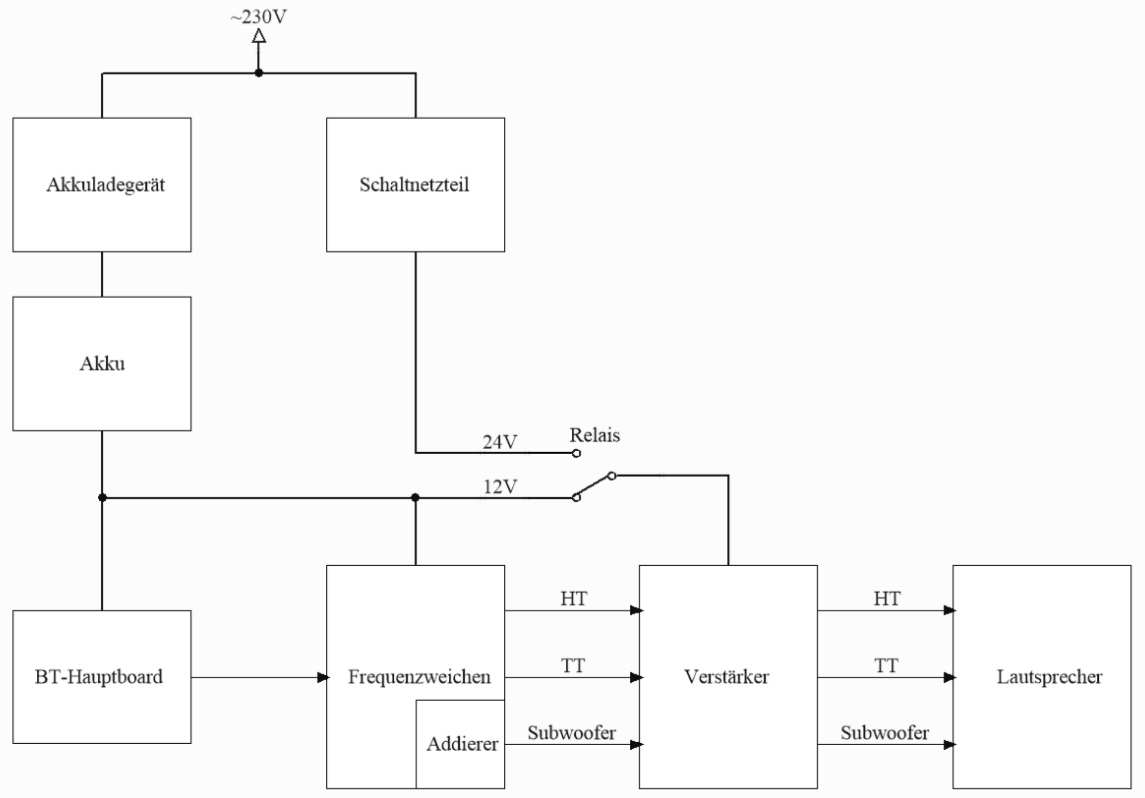
\includegraphics[width=1\textwidth]{img/blockschaltbild.png}
	\caption{Blockschaltbild}
	\label{fig:3.1.1}
\end{figure}
Ein wichtiger Teil des Projekts ist die Bluetooth-Hauptplatine (in Abb. \ref{fig:3.1.1} links unten).
Diese Platine verfügt über die Audio-Eingänge des Projekts.
Das Stereo-Audio-Signal kann mithilfe der BT-Hauptplatine mittels Klinkenbuchse oder Übertragung über Bluetooth (siehe: Kap. \ref{sec:3.3}) in die gesamte Schaltung eingespeist werden.
\\ \\
Dieses Stereo-Audio-Signal wird dann mithilfe der Frequenzweichen in 3 verschiedene Frequenzbereiche (Hochton-, Mittel-Tiefton- und Bassbereich) aufgetrennt.
\\
Tiefe Frequenzen (<150Hz) werden \enquote{L + R} (Stereo) addiert und über eine Mono-Tiefpass-Weiche gefiltert.
\\
Insgesamt gibt es dann also 5 Signale, die weiterverarbeitet werden:
\\ 
\begin{itemize}
	\item Hochton-Links
	\item Hochton-Rechts
	\item Mittel-Tiefton-Links
	\item Mittel-Tiefton-Rechts
	\item Mono-Bassbereich
\end{itemize}

Die verschiedenen Audio-Signale werden dann mit je einem Leistungs-Verstärker verstärkt.
Die Ausgangsleistung der Leistungs-Verstärker variiert je nach Frequenzbereichen.
Dies ist bedingt durch die verwendete Verstärkerschaltung.\\
Diese Schaltungen sind für:
\begin{itemize}
	\item \textbf{Hochtonbereich:}\\ TDA2030-Leistungsverstärker-Grundschaltung
	\item \textbf{Mittel-Tieftonbereich:}\\ TDA2030-Leistungsverstärker mit Leistungstransistoren
	\item \textbf{Bassbereich:}\\ TDA2030-Leistungsverstärker mit Leistungstransistoren in H-Brücke
\end{itemize}
Aus diesen Schaltungen erschließen sich folgenden maximale Ausgangsleistungen, bei asymmetrischer Spannungsversorgung von 24V und 1\% Klirrfaktor:\\
\begin{itemize}
	\item Hochton-Leistungsverstärker (an 8 Ohm): < 6W
	\item Mittel-Tiefton-Leistungsverstärker (an 4 Ohm): < 11W
	\item Bassbereich-Leistungsverstärker (an 4 Ohm): < 44W
\end{itemize}

Versorgt wird die Elektronik mit unter Akkubetrieb mit 12 V oder 24 V unter Netzbetrieb, genauere Erklärung im Kapitel \ref{sec:3.4}.
Somit befindet man sich an der Untergrenze der Leistungs-Verstärker-Schaltungen, diese sind maximal bis \enquote{+/- 22V} oder \enquote{+ 44V asymmetrisch} ausgelegt.
%Da eine Blei-Vlies-Batterie für das Projekt vorgesehen war und diese zumeist 12V liefern, ist die Entscheidung von einer 12V Spannungsversorgung sehr nahe.
%Andere Alternativen wie zB. LiPo-Akkus könnten mehr Spannung und Strom liefern, diese sind jedoch um einiges vorsichtiger zu Behandeln (sehr hohe Energiedichte) und daher auch umständlicher (Lade-Überwachung, Brandgefahr).

\newpage
\section{Mehrweg-Lautsprechersysteme}\label{sec:3.2}
Ein Lautsprecher ist ein Bauelement, das ein elektrisches Signal in ein akustisches Signal (20 Hz bis 20 kHz) umwandelt.
Dabei wird eine Membran in Schwingung versetzt, die wiederum die umgebende Luft zum Schwingen bringt und einen hörbaren Ton erzeugt.
\\ \\
Nun wird aber nicht jede Frequenz gleich gut von ein und demselben Lautsprecher abgestrahlt.
Durch die physikalischen Gegebenheiten strahlen große Membranen tiefe Frequenzen besser ab als hohe Frequenzen.
Daher ist es sinnvoll, mehrere Lautsprecher für verschiedene Frequenzbereiche zu verwenden.
Benannt werden diese verschiedenen Lautsprecher durch den Bereich in dem sie am besten funktionieren.
Beispielsweise Hochton-Lautsprecher oder Hochtöner für den Hochton-Bereich (>2,5 kHz).
Wie gut nun verschiedene Frequenzen von einem Lautsprecher abgestrahlt werden, ist in seinem Frequenzgang ersichtlich:
\begin{figure} [H]
	\centering
	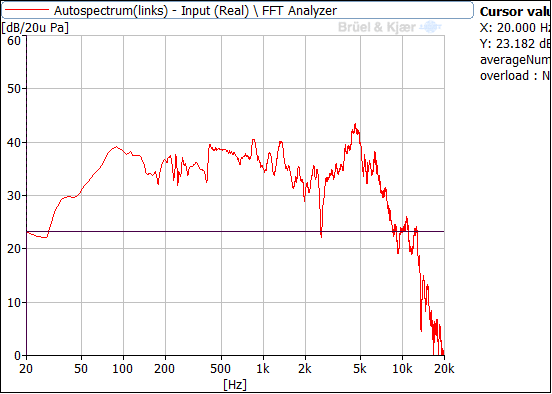
\includegraphics[width=1\textwidth]{img/LSMessung/TT1_9,17l_bestes.png}
	\caption{Beispiel eines Frequenzganges (Tieftöner PSS 297 58206)}
	\label{fig:3.2.1}
\end{figure}
Bei einem perfekten Lautsprecher würde diese Linie (Abb. \ref{fig:3.2.1}) eine parallele Gerade zur X-Achse bilden.
Da so ein Lautsprecher aber nicht existiert, werden verschiedene Frequenzen auch mit einem verschiedenen Schalldruckpegel vom Lautsprecher abgestrahlt.
\\
In dem Beispiel (Abb. \ref{fig:3.2.1}) wurde ein Tieftöner gemessen.
Das ist klar ersichtlich, da der Schalldruckpegel ab 5 kHz fast kontinuierlich fällt.
Tiefere Frequenzen werden, in einem gewissen Bereich, gleich wiedergegeben.
\\ \\
Je nach Frequenzbereich kann ein Ton vom menschlichen Ohr auch lokalisiert \mbox{werden}.
Hohe Frequenzen (<20 kHz) sind besser lokalisierbar als tiefe Frequenzen.
Bei sehr niedrigen Frequenzen (<150 Hz) ist der Ton gar nicht mehr lokalisierbar.
Diesen \mbox{Effekt} kann man nutzen und damit akustische Effekte erzeugen.
Einige Lautsprecher-Systeme, die diesen Effekt nutzen sind:
\begin{itemize}
	\item 2.0-System
	\item 2.1-System
	\item 5.1-System
\end{itemize}
Dabei steht die erste Zahl für die Anzahl der verteilten Lautsprecher und die zweite Zahl für die Anzahl der verwendeten Subwoofer.
\\
Je mehr verteilte Lautsprecher benutzt werden, desto bessere Raumklang-Effekte sind realisierbar.
Dadurch wird die Beschaltung aber auch komplizierter, da 5 verschiedene Audio-Signale verwendet werden.
\\ \\
Der Subwoofer ist ein spezieller Lautsprecher.
Er arbeitet im Bass-Bereich(20-150 Hz) und verarbeitet nur ein einziges Signal.
Diese Frequenzen sind nicht lokalisierbar, weshalb auch nur ein Subwoofer benötigt wird.
Meistens ist die Membran des Subwoofers um einiges größer als die Membran der anderen Lautsprecher.
Damit kann der Subwoofer mehr Luft in Bewegung setzen und somit einen höheren Schalldruckpegel erzeugen.
Um das zu ermöglichen benötigt der Subwoofer aber auch mehr Leistung als die anderen Lautsprecher.
\\ \\
In unserem Projekt haben wir uns direkt für ein 2.1-System entschieden, da sich dieses System am besten bewährt hat und für Musik ein Stereo-System völlig ausreicht.
Die zwei verteilten Boxen, auch Satelliten genannt, sind mit je einem Hochton- und einem Tiefton-Lautsprecher ausgestattet und werden über Kabeln mit der Hauptbox verbunden.
Damit sollen die Satelliten fast den gesamten Frequenzbereich für Audio (20 Hz bis 20 kHz) abdecken.
Der einzelne Subwoofer übernimmt den Bass-Bereich (<150 Hz) und sitzt in der Hauptbox.
Dort ist auch die gesamte Elektronik verbaut.

\section{Signalübertragung über Bluetooth}\label{sec:3.3}
Bluetooth ist eine moderne Funkschnittstelle für verschiedenste Anwendungen.
Unter anderem gibt es auch speziell für Audio-Anwendungen konzipierte Protokolle.
Die Übertragung läuft folgendermaßen ab:
\\
Zuerst muss das sendende Gerät (z.B. ein Smartphone) mit dem empfangenden Gerät (z.B. Bluetooth-Modul) verbunden werden.
Danach werden die gewünschten Daten ausgewählt.
In diesem Fall wären die Daten ein Musikstück.
Über Funk werden die digitalen Daten an das empfangende Gerät gesendet.
Nun muss das Bluetooth-Modul diese digitalen Daten wieder in ein analoges Signal umwandeln, welches dann weiterverarbeitet werden kann.
\\ \\
Dabei ist eine hohe Kompatibilität mit viele Geräten wichtig, weil es sehr viele verschiedene Versionen von Bluetooth gibt.
Da Bluetooth-Geräte meist abwärtskompatibel sind, ist es sinnvoll das Modul mit einer älteren BT-Version laufen zu lassen.
\\ \\
Nach ausführlicher Recherche wurde das Modul \enquote{XS3868} ausgewählt.
Der darauf verbaute Chip \enquote{OVC3860} von \enquote{OmniVision Technologies} hat sich bereits in vielen anderen Projekten bewährt, da er günstig ist und Funktionen wie \enquote{Play/Pause} bereitstellt.
\newpage
Im \enquote{OVC3860} (Abb. \ref {fig:3.3.1}) ist außer der Bluetooth-Verbindung auch noch ein Stereo-Audio-Prozessor verbaut.
Zusätzlich gibt es noch eine UART-Schnittstelle mithilfe man einige Einstellungen am Chip vornehmen kann.
Eine LiPo-Akku-Ladeschaltung ist ebenfalls vorhanden, wird aber in diesem Projekt nicht verwendet.
\\
Das Modul benötigt eine Versorgungsspannung von 3,3 V bis 4,2 V, wobei der Chip mit 1,8 V versorgt wird.
Diese Spannung (1,8 V) wird auf dem Modul erzeugt.
\\
Die verwendete BT-Version ist 2.0.
Einige GPIO-Pins sind auf das Modul herausgeführt um Funktionen wie \enquote{Play/Pause} zu ermöglichen.
Der Chip benötigt einen externen Speicher und eine Antenne (auf dem Modul) um ordnungsgemäß zu funktionieren.
\begin{figure} [H]
	\centering
	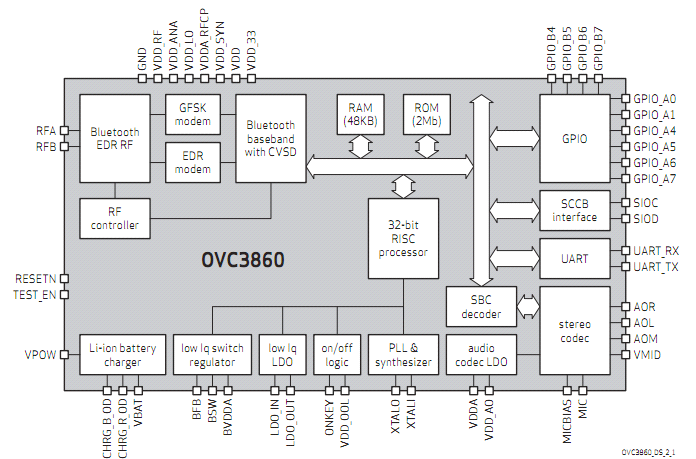
\includegraphics[width=1\textwidth]{img/BTModul/blockschaltbild.png}
	\caption[Blockschaltbild OVC3860]{Blockschaltbild OVC3860\footnotemark}\label {fig:3.3.1}
\end{figure}
\footnotetext{http://cxem.net/review/files/review24\_OVC3860.pdf,\\Zugriff: 11.03.2017}

\newpage
\section{Spannungsversorgung}\label{sec:3.4}
Die gesamte Box soll portabel sein, d.h. ohne externe Stromzufuhr funktionieren.
Dafür ist ein Akku notwendig.
Nach einigen Überlegungen haben wir uns für einen Blei-Vlies-Akku entschieden.
Gründe dafür sind:
\begin{itemize}
	\item Geringe Kosten
	\item Einfache Beschaltung
	\item Geringere Gefahr gegenüber Lithium-Akkus
	\item Wegen Vlies-Technik: Kein Auslaufen von chemischen Substanzen
\end{itemize}
Dieser Akku versorgt grundsätzlich die Elektronik mit 12 V und wird über ein passendes Ladegerät aufgeladen.
Da aber mit dieser, relativ geringen, Spannung nur eher kleine Leistungen zu erwarten sind, kam die Idee auf, die Verstärker bei externer Versorgung durch das Stromnetz (230 V / AC) mit einer größeren Spannung (24 V) zu versorgen.
Um das zu realisieren wird ein Netzteil, in unserem Fall ein Schaltnetzteil benötigt.
Falls das Gerät am externen Stromnetz hängt, wird die Versorgung der Verstärker automatisch mithilfe eines passenden Relais umgeschaltet.
Diese Lösung wurde gewählt, da sie sehr simpel ist und gut funktioniert.
Veranschaulicht wird das Konzept durch diese Schaltung:
\begin{figure} [H]
	\centering	
	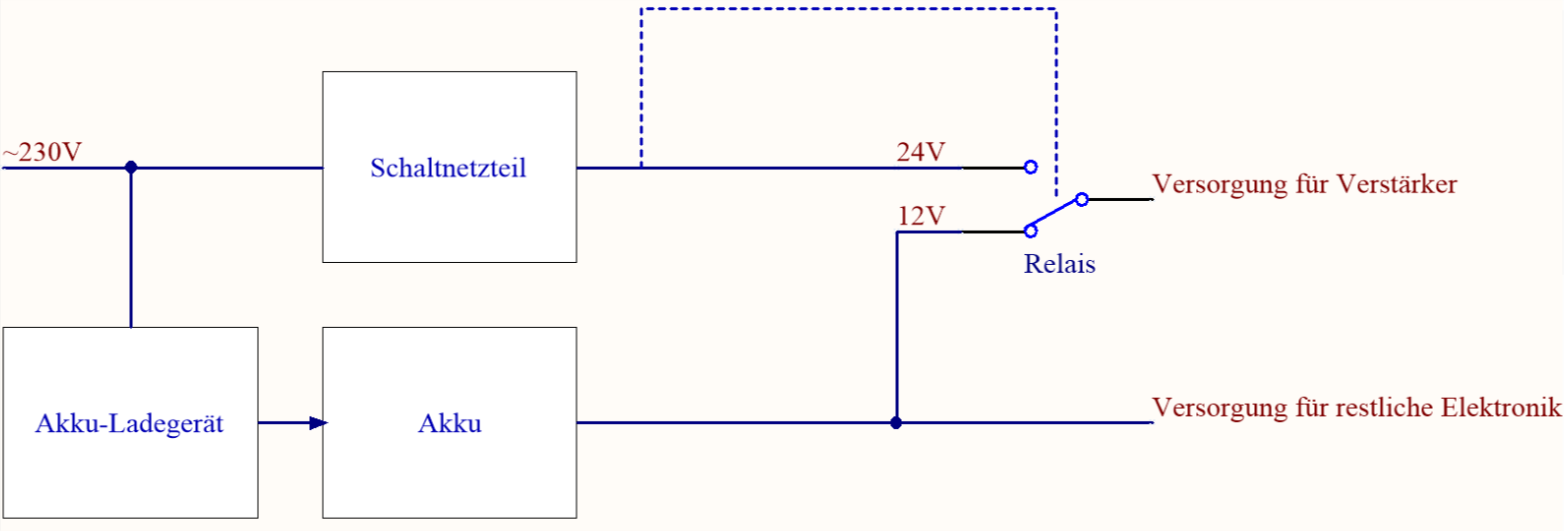
\includegraphics[width=1\textwidth]{img/Grundlagen/Versorgung.png}
	\caption{Versorgungskonzept}
	\label {fig:3.4.1}
\end{figure}
Das Lautsprecher-System kann somit bei Netzbetrieb die Musik lauter abspielen, als bei Akku-Betrieb.

% ANDERE VERSION
%Da das Projekt portabel sein soll, ist auch ein Akku (Vlies-Blei-Akku) eingebaut.
%Er versorgt die gesamte Elektronik mit 12 V bei Akkubetrieb.
%Aufgeladen wird er durch ein passendes Ladegerät, welches aber nicht von uns entwickelt wird.
%\\ \\
%Falls eine externe Stromversorgung über eine Steckdose (230V AC) gegeben ist, ändert sich die Versorgung der Verstärker.
%Während nun der Akku aufgeladen wird, schaltet ein Relais die Versorgungsspannung der Verstärker von 12 V auf 24 V um.
%Diese Spannung (24 V) wird durch ein Schaltnetzteil erzeugt.
%\\ \\
%Durch eine höhere Spannung können die Verstärker auch die Signale auf höhere Spannungen verstärken.
%Somit ergibt sich eine höhere Leistung an den Verstärkern aber auch an den Lautsprechern.
%Eine Leistungssteigerung an einem Lautsprecher entspricht einer Steigerung des Schalldruckpegels was wiederum eine höhere Lautstärke bewirkt.
%An den Verstärkern bewirkt eine höhere Leistung auch eine größere Wärmeentwicklung.
%Der verbaute Kühlkörper muss diese Wärme bei Akkubetrieb als auch bei Netzbetrieb ableiten können.
%\\ \\
%Das Lautsprecher-System kann somit bei Netzbetrieb die Musik lauter abspielen, als bei Akku-Betrieb.


% Technische Erklärung und Messungen
\chapter{Realisierung und Ergebnisse}
\responsible{Andreas Macsek}
\subsection{Mono-Bass-Addier-Schaltung und Mono-Bass-Weiche}
\subsubsection{Allgemeines}
Das empfangene Audio-Signal muss für das Lautsprecher-System aufgetrennt werden. In Hoch, Mitte und Tief Audiofrequenz. Für den \enquote{Mono-Bass} werden die tiefen Frequenzen aus dem Signal heraus gefiltert. Da, wie der Name schon sagt, es sich um einen \enquote{Mono-Bass} handelt, muss das Stereo-Audio-Signal vorher noch mittels OPV-Addierschaltung addiert werden um ein Mono-Audio-Signal zu erhalten.


\subsubsection{Zielsetzung}
Es soll ein Print angefertigt werden, welcher über eine OPV-Addierschaltung verfügt und des weiteren das eintreffende Audio-Signal über ein Filter passend für den \enquote{Mono-Bass} filtert.
Diese Schaltung für das Tiefpass-Filter muss variabel designet werden. Das Tiefpass-Filter muss unabhängig vom Printdesign, nur durch Ändern von Bauteilwerten, andere Grenzfrequenzen liefern können.




\subsubsection{Auswahl des Tiefpass-Filters}
Es wurde nach einem möglichst steilen, im Durchlassbereich linearen und einfachen Tiefpass-Filter gesucht. Man hat sich nach Überlegen für ein \enquote{Aktives-Tiefpass-Filter 2.Ordnung} entschieden, dabei wurde die \enquote{Butterworth-Schaltung} bevorzugt. Wegen seiner hohen Linearität im Durchlassbreich und einer Dämpfung von $\frac{-20dB}{Dek.}$ . Dies bedeutet, dass eine Frequenz die 10mal größer ist als die Grenzfrequenz einen um $\frac{1}{10}$ kleineren Pegel aufweist, als die Grenzfrequenz.\\
Zur Regelung wird an den Eingängen (Rechts, Links) und am Ausgang der Schaltung jeweils ein Potentiometer in der Größenordnung von 1kOhm verbaut. Diese dienen zur Anpassung der Amplitude des ein- und ausgehenden Signals, um mögliche Übersteuerungen zu vermeiden.

\subsubsection{Butterworth-Filter 2. Ordnung}
Die Grundschaltung eines Butterworth-Tiefpass-Filter 2. Ordnung ist auch bei verschieden Grenzfrequenzen gleich. Es besteht hauptsächlich aus einem OPV, drei Widerständen und zwei Kondensatoren. Deren Anordnung ist ausschlaggebend für das Tiefpass-Filter (Abb. \ref{fig:abb3.1}).\\ 
Bedingt durch das Beschalten des OPVs wird das Ausgangssignal invertiert, was hier keine gröberen Folgen mit sich bringt.\\ 
Am Plus-Eingang des OPVs wird entweder Masse bei symmetrischer Spannungsversorgung, oder $\frac{Vcc}{2}$ bei asymmetrischer Spannungsversorgung angelegt.
\begin{figure} [h]
	\centering
	\caption{Butterworth-Filter 2. Ordnung}
	\label {fig:abb3.1}
	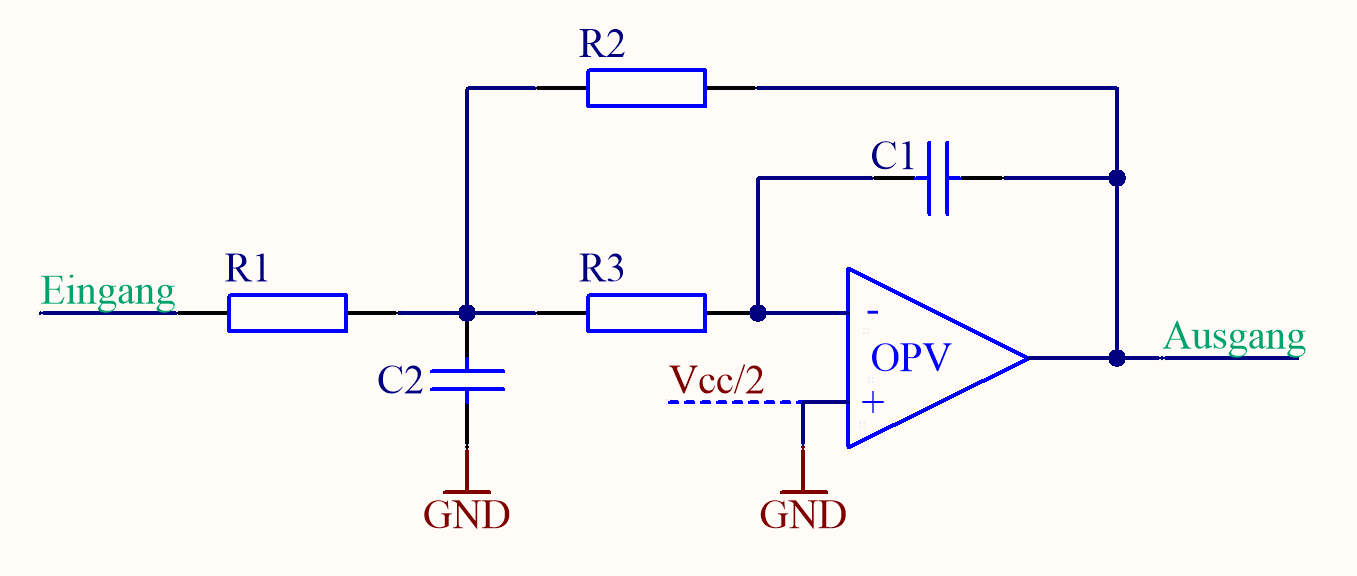
\includegraphics[width=1\textwidth]{img/TPFilterButterworth2Ordnung.PNG}
\end{figure}\\

\subsubsection{Schaltung}
Passend dem Signalverlauf sitzt am Beginn der Schaltung (Abb. \ref{fig:abb3.2}) die erste Regelung über Potentiometer. Anschließend kommt man zu der Addier-Schaltung (Abb. \ref{fig:abb3.3}) welche das Stereo-Signal in ein Mono-Signal wandelt und dadurch Stereo-Effekte wie zB. Balance am \enquote{Mono-Bass} entfernt.\\
Wichtig ist bereits hier die Versorgung der Schaltung. Bedingt durch eine asymmetrische Spannungsversorgung (0...12V) muss am OPV ein Arbeitspunkt eingestellt werden. Dabei handelt es sich um ein absichtliches Anheben des Signals in Y-Richtung bei einem Spannungs-Zeit-Verlauf, sodass die untere Halbwelle des Signals nicht verloren geht. Dafür muss am Plus-Eingang des OPVs der Addier-Grundschaltung und der Butterworth-Filter-Schaltung die halbe Versorgungsspannung angelegt werden, um das beste Ergebnis zu erzielen. Dafür wird an den beiden Plus-Eingängen der OPVs über eine Spannungsteiler-Schaltung aus zwei Widerständen das benötigte $\frac{Vcc}{2}$ angelegt.\\
Um Störungen im OPV zu vermeiden wird sehr nahe an diesem ein 10µF ELKO in der Versorgungsspannungsleitung vorgesehen.\\
Nach Addieren des Stereo-Signals zu einem Mono-Signal kommt dieses zum Aktiven-Tiefpass-Filter(Abb. \ref{fig:abb3.4}). Bevor das gefilterte Signal weiter zum Verstärker geht wird nochmals die Möglichkeit geboten um die Amplitude des Signals anzupassen.
\begin{figure} [h]
	\centering
	\caption{Schematic Mono-Bass-Addier-Schaltung und Mono-Bass-Weiche}
	\label {fig:abb3.2}
	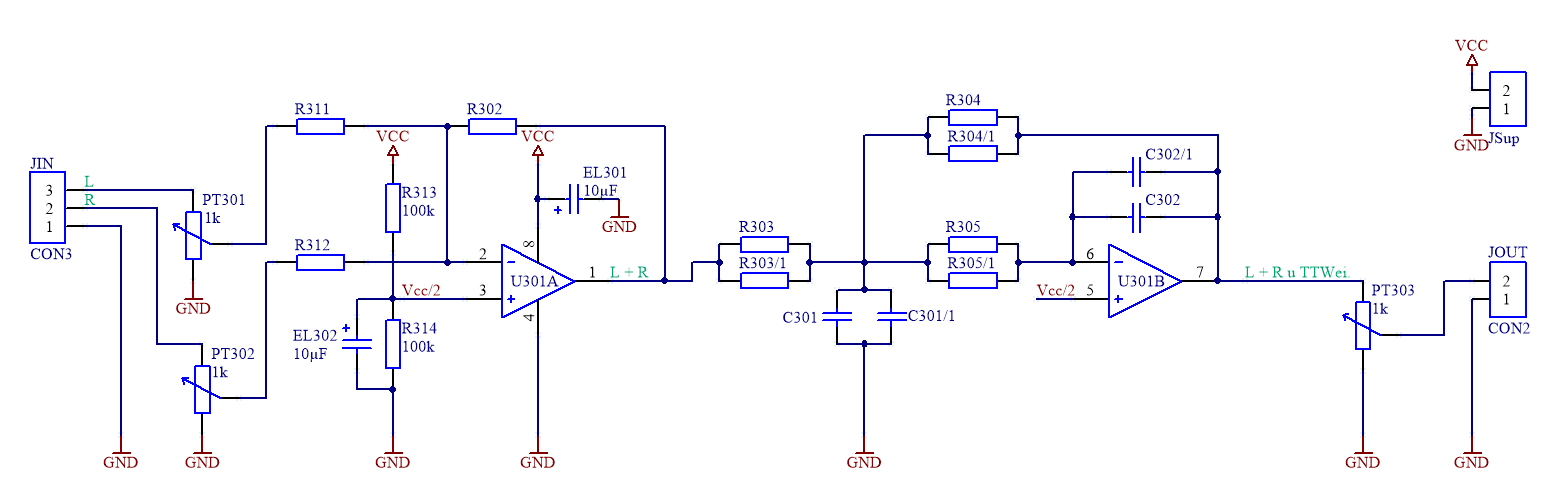
\includegraphics[width=0.8\textwidth]{img/3mTTWeicheruAddiererDiplSchematic.PNG}
\end{figure}
\begin{figure} [h]
	\centering
	\caption{Schematic Mono-Bass-Addier-Schaltung}
	\label {fig:abb3.3}
%	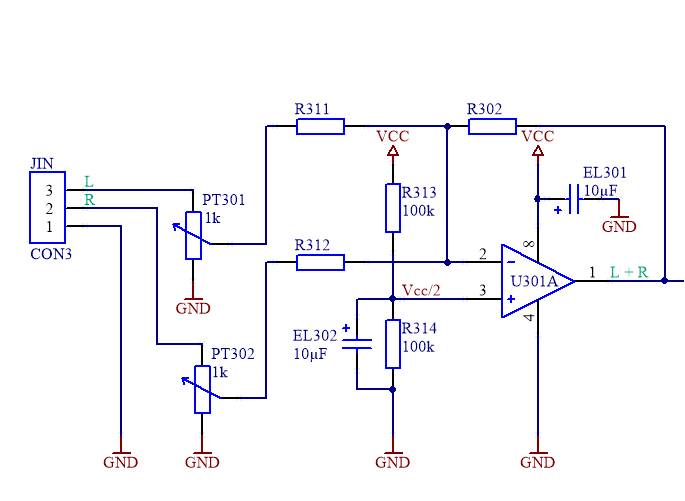
\includegraphics[width=0.8\textwidth]{img/3mTTWeicheruAddiererDiplSchematicTeil1.png}
\end{figure}
\begin{figure} [h]
	\centering
	\caption{Schematic Mono-Bass-Weiche}
	\label {fig:abb3.4}
%	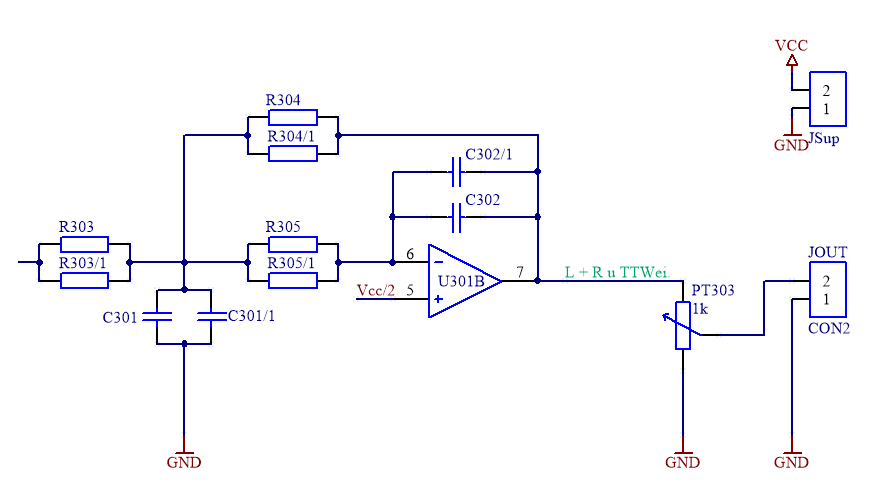
\includegraphics[width=0.8\textwidth]{img/3mTTWeicheruAddiererDiplSchematicTeil2.png}
\end{figure}



\subsubsection{PCB}
An einer der vier Seiten der Leiterplatte(Abb. \ref{fig:abb3.5}) wurden alle wesentlichen Ein- und Ausgänge platziert. Eine dreipolige Eingangsstiftleiste für Rechts, Links und Masse. Eine zweipolige Ausgangsstiftleiste für Signal und Masse. Des weiteren darf die Spannungsversorgung nicht fehlen. Wegen größeren Spannungen wurden massivere Stecker verwendet. In diesem Fall handelt es sich um Pol-Klemmen. Zum testen wurde ein zusätzlicher Masse-Printstift angebracht um bei Messungen mit einem Oszilloskop einem besseren Massebezugpunkt zu haben.\\
Die Bauteile wurden nach Möglichkeit gestaffelt, beziehungsweise gruppiert auf der Leiterplatte platziert um den Platzbedarf zu minimieren.
\begin{figure} [h]
	\centering
	\caption{PCB}
	\label {fig:abb3.5}
	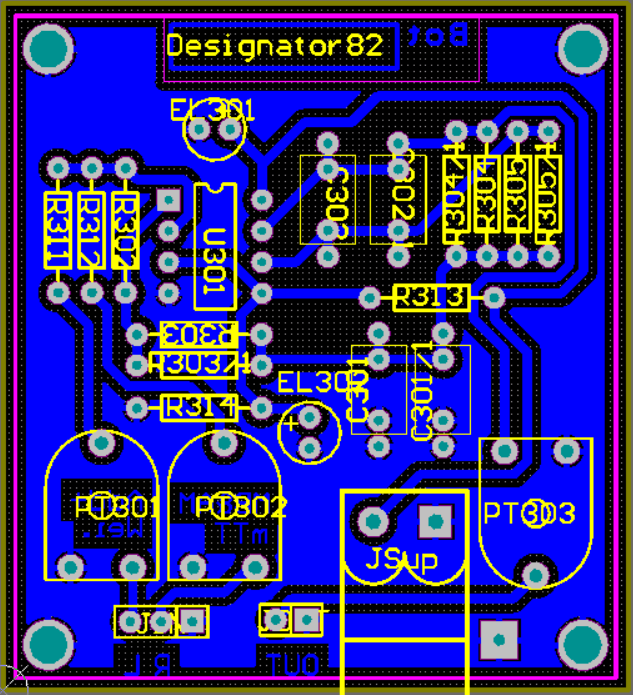
\includegraphics[width=0.8\textwidth]{img/3mTTWeicheruAddierer-PCB.PNG}
\end{figure}



\begin{comment}
%% Altium und Einstellungserklärung + Wichtige Layout-Faktoren
%Beim designen des Leiterplattenlayouts wurden die allgemeinen Altium-Einstellungen vorgenommen und auf die zu berücksichtigenden Layoutpunkte geachtet.
Beim \enquote{Layouten} der Schaltung mussten einige wichtige Faktoren berücksichtigt werden.\\
Wie da wären:\\
\begin{itemize}
	\item EMV-Technische-Faktoren, wie kurze Leiterbahnen
	\item Ausnützen der Printfläche
	\item Mehrfach-Footprints ermöglichen für verschiedene Bauteile
	\item Mechanische Aufhängebohrungen vorsehen
	\item Massefläche bei Möglichkeit vorsehen
\end{itemize}\\
Leiterplattenspezifische Einstellungen wurden aus den Kriterien der schuleigenen Leiterplattenfertigung übernommen. Zu diesen Einstellungen zählen:\\
\begin{itemize}
	\item Leiterbahnbreite
	\item Leiterbahnabstände untereinander
	\item Restring bei Bohrungen
	\item 
\end{itemize}
\end{comment}




%%\begin{comment}

\subsubsection{Inbetriebnahme}
Bereits mit einer simplen Beschaltung kann das Modul in Betrieb genommen werden:
\begin{figure} [h]
	\centering
	\caption{Prinzipschaltung XS3868}
	\label {fig:abb2.3}
%%	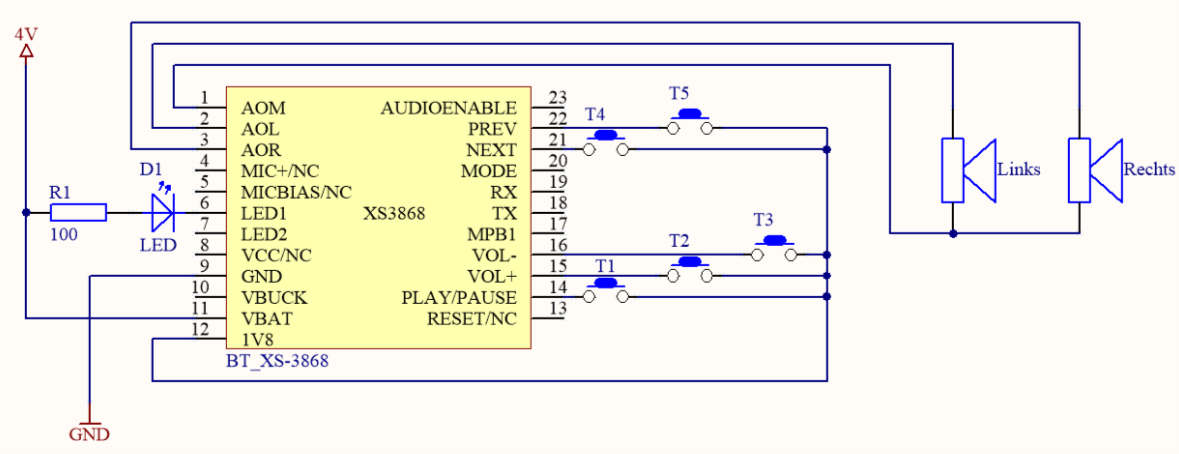
\includegraphics[width=1\textwidth]{schaltungen/XS3868_Prinzipschaltung.png}
\end{figure} \\
Mit dieser Schaltung (Abb. \ref {fig:abb2.3}) kann das Modul bereits ordnungsgemäß arbeiten.\\
Die Versorgungsspannung ist mit 4V etwas höher gewählt damit es nicht zu Ausfällen durch Spannungsschwankungen kommt. Das XS3868-Modul hat eine Stromaufnahme von ca. 30mA beim Starten, 10mA im Stand-By und bis zu 100mA wenn Musik abgespielt wird.\\ \\
Die Status-LED ist, wie in Abbildung \ref {fig:abb2.3} dargestellt, \enquote{Low-Aktiv}. Beim Starten des Moduls und während der Suche nach Geräten blinkt sie durchgehend, wobei sie bei einer bestehenden Verbindung nur die Hälfte der Zeit blinkt.\\ \\
Mit einfachem Betätigen eines Tasters wird die entsprechende Funktion vom Modul ausgeführt, jeweils mit einem Bestätigungston begleitet. Dieser Ton wird auch beim Starten des Moduls abgespielt.\\ \\
Statt die Lautsprecher direkt an das Modul anzuschließen, sollte allerdings noch ein Verstärker verbaut werden.
\newpage


\subsubsection{Verbindung mit dem Modul}
Wenn der OVC3860 eingeschaltet ist, sucht er andauernd nach BT-Geräten. Mit einem Smartphone findet man das Gerät und kann sich mit einem Standard-PIN-Code (\enquote{0000}) verbinden. Wenn bereits Lautsprecher angeschlossen sind, wird ein Ton abgespielt, der die Verbindung bestätigt. Außerdem hat die Status-LED nun ein anderes Blinkverhalten (Mehrmaliges Blinken mit längeren Pausen).\\ \\
Jetzt ist das Modul bereit Musik abzuspielen. Diese kann vom Smartphone oder vom Modul aus gesteuert werden. Die notwendigen Taster müssen allerdings schon in der Schaltung verbaut sein um die Bedienung der Musik zu ermöglichen.


\subsection{Zusatz-Leiterplatten}
\subsubsection{Allgemeines}
Als Entwicklungsprogramm für beide Leiterplatten wurde  \enquote{Altium Designer 13.3} verwendet. Die Schaltung wurde in diesem Programm gezeichnet, das Layout für die Leiterplatten angefertigt und entflechtet. Es wurden einseitige Platinen verwendet, da doppelseitige nicht notwendig waren.


\subsubsection{Adapter-Board}
Da das Modul in SMD-Bauform gefertigt ist, wurde ein Adapter-Board (Abb. \ref{fig:abb3.1}) vorgesehen um eine einfachere Handhabung mit dem Modul zu ermöglichen. Als Anschlussmöglichkeiten werden Stiftleisten verwendet.\\
Die Schaltung ist deshalb auch sehr simpel aufgebaut:
\begin{figure} [h]
	\centering
	\caption{Schaltung des Adapter-Boards}
	%%\label {fig:abb3.1}
%%	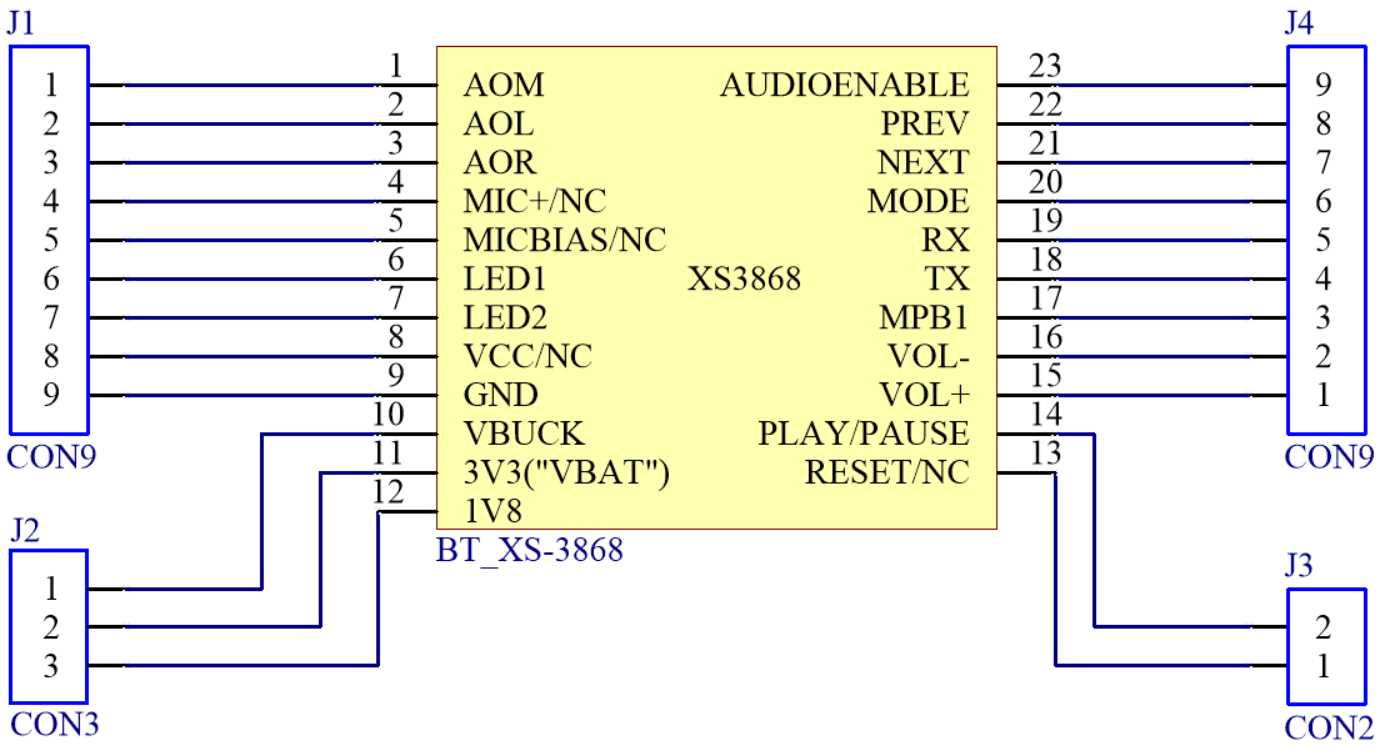
\includegraphics[width=1\textwidth]{schaltungen/adapter_sch.png}
\end{figure} \\
Jeder Pin bekommt auch auf dem Adapter einen eigenen Pin auf der Stiftleiste.
\newpage
Das PCB (Abb. \ref{fig:abb3.2}) ist, wie bereits erwähnt, einseitig aufgebaut:
\begin{figure} [h]
	\centering
	\caption{PCB des Adapter-Boards}
%%	\label {fig:abb3.2}
%%	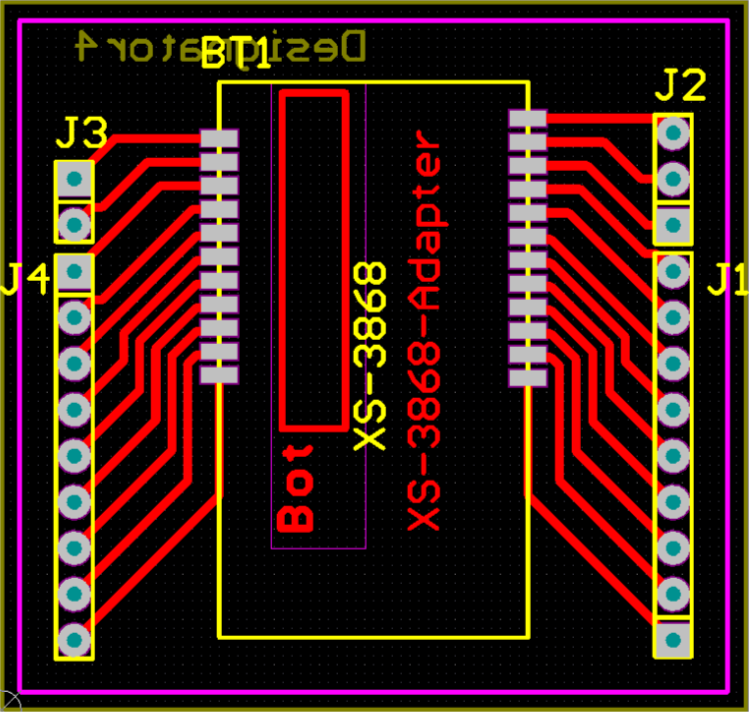
\includegraphics[width=1\textwidth]{schaltungen/adapter_pcb.png}
\end{figure} \\
Mit diesem PCB kann da BT-Modul nun besser getestet und auch weiterverwendet werden. Gemeinsam mit diesem Adapter kommt es auch auf das Hauptboard.
\newpage


\subsubsection{Hauptboard}
\minisec{Funktion}
Das Hauptboard wird hauptsächlich zur Versorgung des BT-Moduls, aber auch zur Weiterverarbeitung des Audio-Signals verwendet. Darüber hinaus ist eine Additionsschaltung vorgesehen, die das Signal des BT-Moduls mit einem zweiten, von einem Klinken-Eingang zugeführten, Signal vermischt. Die Lautstärke von diesem zweiten Audio-Signal kann über ein Stereo-Potentiometer geregelt werden. \\
Weiterhin sind die Pins zur Bedienung der Musik an einen 2x5-Wannenstecker herausgeführt. Zugang zur seriellen Schnittstelle wird auch ermöglicht.

\minisec{Schaltung}
Die Schaltung (Abb. \ref{fig:abb3.3}) des Hauptboards ist in mehrere Teile aufgeteilt und wird deshalb auch einzeln erklärt.
\begin{figure} [h]
	\centering
	\caption{Schaltung des Hauptboards (Versorgung + BT-Modul)}
%%	\label {fig:abb3.3}
%%	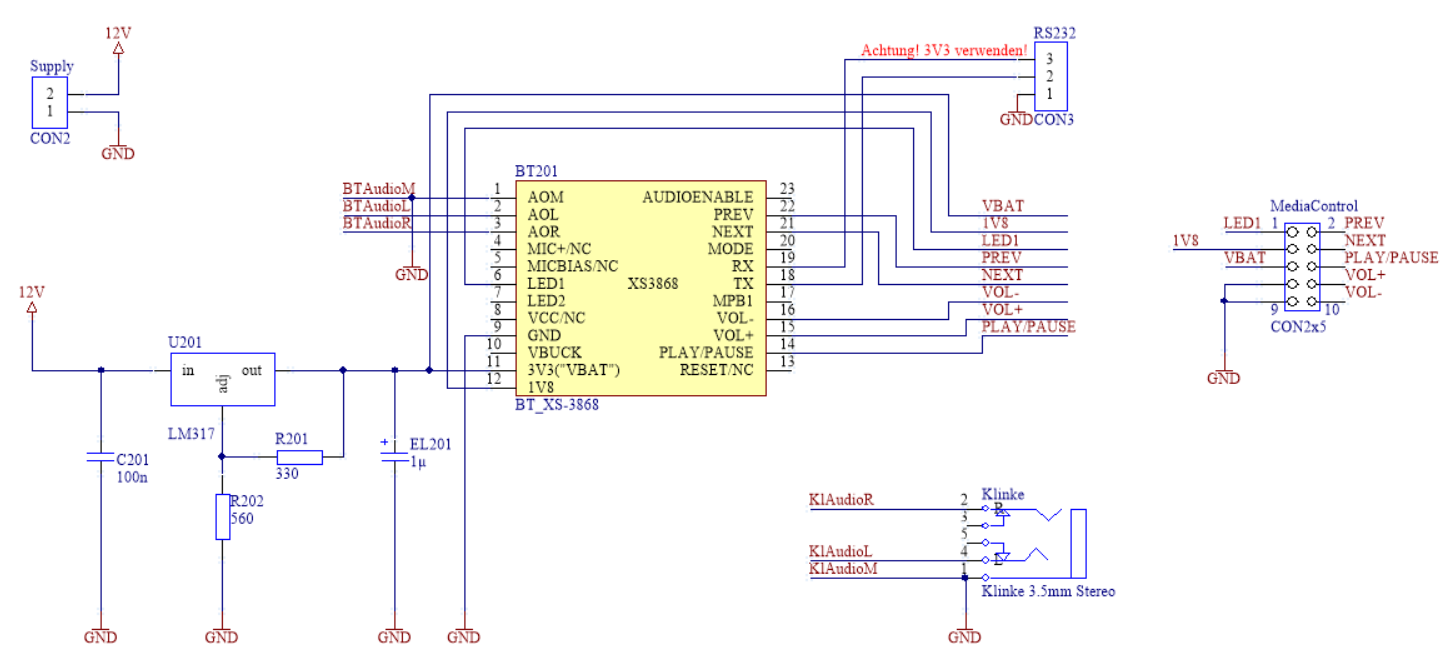
\includegraphics[width=1\textwidth]{schaltungen/hauptboard_sch1.png}
\end{figure} \\
In diesem Teil der Schaltung ist zu sehen: die Versorgungsbuchse, die Versorgungsschaltung für das BT-Modul, das BT-Modul mit herausgeführten Pins und die Klinken-Buchse.\\
Der Spannungsregler LM317 (Bezeichnung: U201) stellt eine Versorgungsspannung von 3,9V für das BT-Modul ein. Mit einer maximalen Stromaufnahme von 100mA ergibt sich folgende Verlustleistung:
\begin{equation}
	P_{max} = 7,9V * 100mA = 0,79W
\end{equation}
Deshalb wird auch kein Kühlkörper benötigt, es wird aber trotzdem eine Alu-Platte an den LM317 geschraubt um sicher zu gehen. \\
Ein eigener Stecker (Stiftleiste) für die Versorgung (12V) sowie die UART-Schnittstelle (RS232) sind auch vorgesehen. Der Wannenstecker (hier: \enquote{MediaControl}) ist mit allen wichtigen Pins des Moduls verbunden und verbindet eine Frontplatine mit dem Hauptboard. \\ \\
Die Klinkenbuchse wird in der folgenden Additionsschaltung(Abb. \ref {fig:abb3.4}) weiterverwendet:
\begin{figure} [h]
	\centering
	\caption{Schaltung des Hauptboards (Additionsschaltung)}
%%	\label {fig:abb3.4}
%%	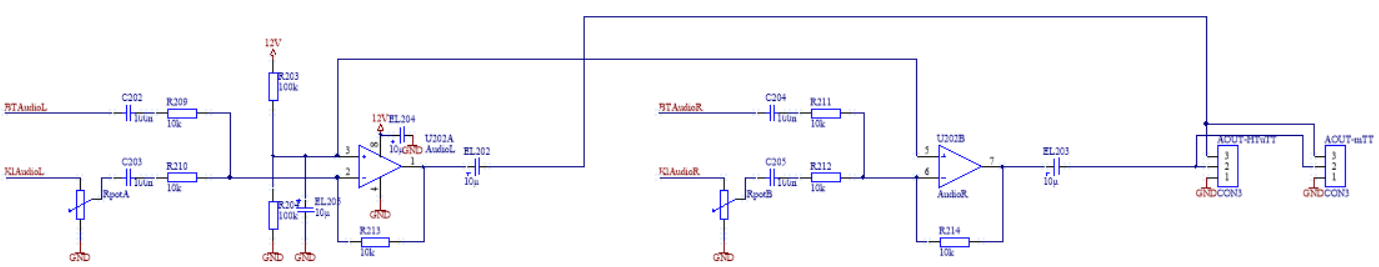
\includegraphics[width=1\textwidth]{schaltungen/hauptboard_sch2.png}
\end{figure} \\
Vergrößert:
\begin{figure} [h]
	\centering
	\caption{Schaltung des Hauptboards (linker Teil der Additionsschaltung)}
%%	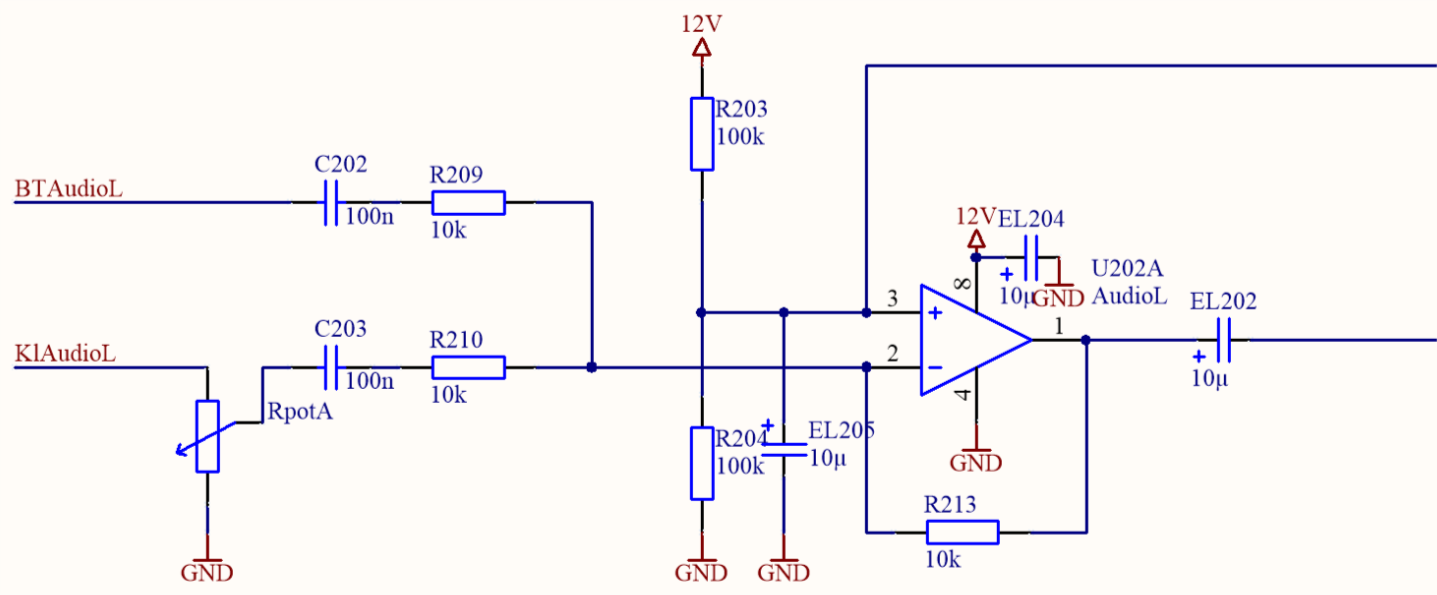
\includegraphics[width=1\textwidth]{schaltungen/hauptboard_sch2_zoom.png}
\end{figure} \\
Mithilfe dieser OPV-Schaltung werden die zwei Audio-Signale (ein Addierer pro Kanal) addiert. Das Signal vom Klinkeneingang kann zuvor noch mit einem Potentiometer abgeschwächt werden.\\
Der Arbeitspunkt bei 6V am Pin 3 wird benötigt um am Ausgang eine Spannung von $\pm$6V zu erreichen. Der OPV wird hier als invertierender Verstärker mit Verstärkung 1 aufgebaut, aber er addiert hier die zwei Signale zusammen auf ein Ausgangssignal.

\minisec{PCB}
Die Platine(Abb. \ref {fig:abb3.6}) für das Hauptboard sollte möglichst kompakt sein und alle Eingänge oder Bedienelemente auf einer Seite (hier rechts) haben. Das BT-Modul wird samt Adapter auf zwei Stiftleisten gesteckt. Darunter werden keine Bauteile verwendet, weil es sonst zu eng wäre. Des weiteren wären Bauteile unter dem Adapterprint während der Testphase unvorteilhaft, da diese schwerer zugänglich sind.
\begin{figure} [h]
	\centering
	\caption{PCB des Hauptboards}
%%	\label {fig:abb3.6}
	%%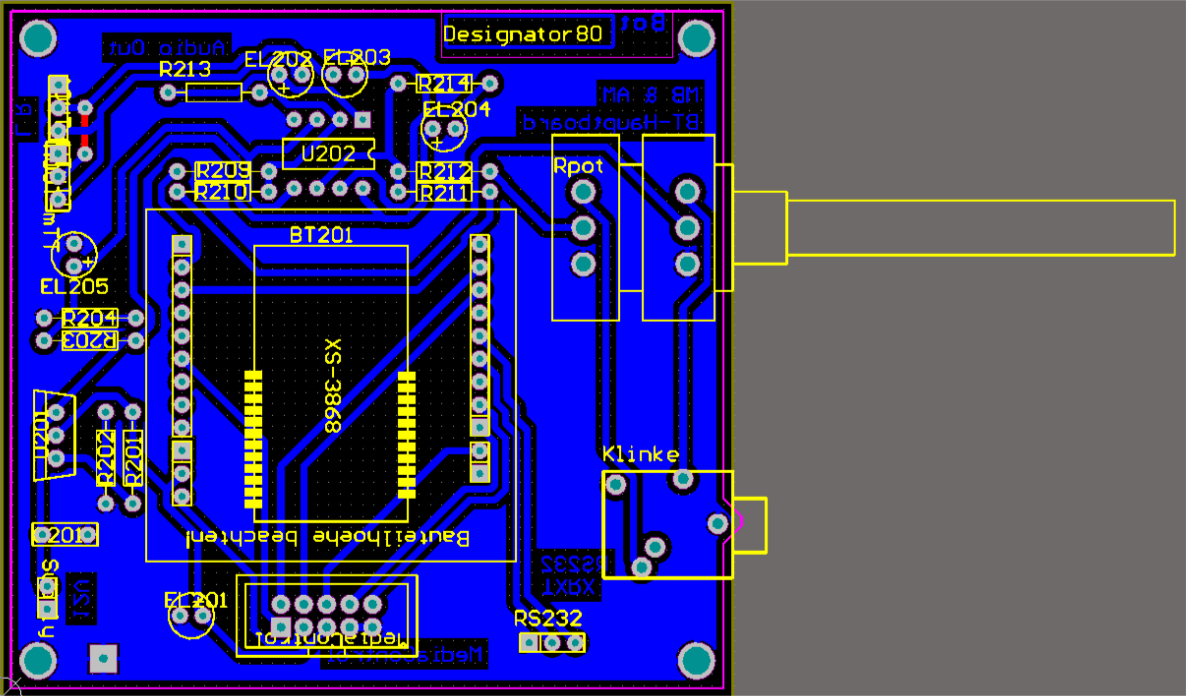
\includegraphics[width=1\textwidth]{schaltungen/hauptboard_pcb.png}
\end{figure}
\newpage


\subsubsection{Frontplatine}
\minisec{Funktion}
Diese Platine ist eigentlich eine Erweiterung des Hauptboards. Es wird mit dem Hauptboard über einen 2x5-Wannenstecker verbunden und auch versorgt. Sonst sind nur die Taster zur Bedienung des BT-Moduls, sowie die Status-LED verbaut.

\minisec{Schaltung}
Die Taster werden jeweils mithilfe eines Kondensators entprellt. Die Höhe der Taster reicht über die Kondensatoren hinaus um eine Bedienung zu ermöglichen. (Abb. \ref{fig:abb3.7})
\begin{figure} [h]
	\centering
	\caption{Schaltung der Frontplatine}
%%	\label {fig:abb3.7}
	%%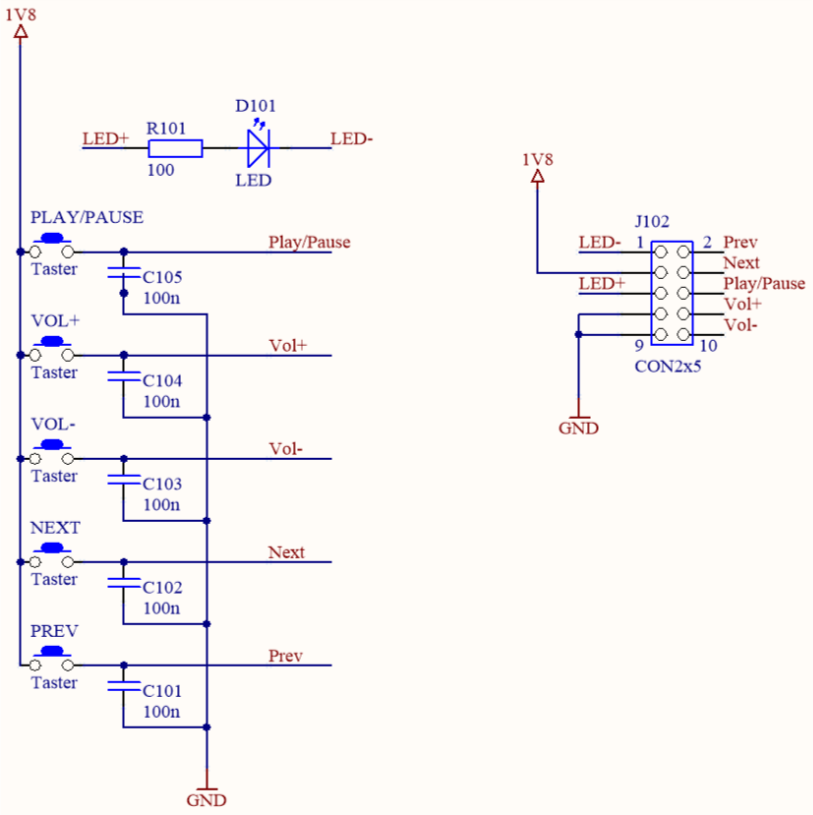
\includegraphics[width=0.7\textwidth]{schaltungen/front_sch.png}
\end{figure} \\
Jeder der Taster ist mit dem 1,8V-Pin des Moduls verbunden und geht dann weiter auf den entsprechenden Funktionspin. Die Bezeichnung \enquote{LED+} entspricht der Versorgungsspannung (\enquote{VBAT} = 3,9V) des Moduls. \enquote{LED-} ist mit dem Ansteuerungssignal am BT-Modul verbunden (Pin 6).

\minisec{PCB}
Das PCB (Abb. \ref {fig:abb3.8}) der Frontplatine soll ebenfalls so klein wie möglich aber von der Bedienung her sinnvoll aufgebaut sein.
\begin{figure} [h]
	\centering
	\caption{PCB der Frontplatine}
%%	\label {fig:abb3.8}
	%%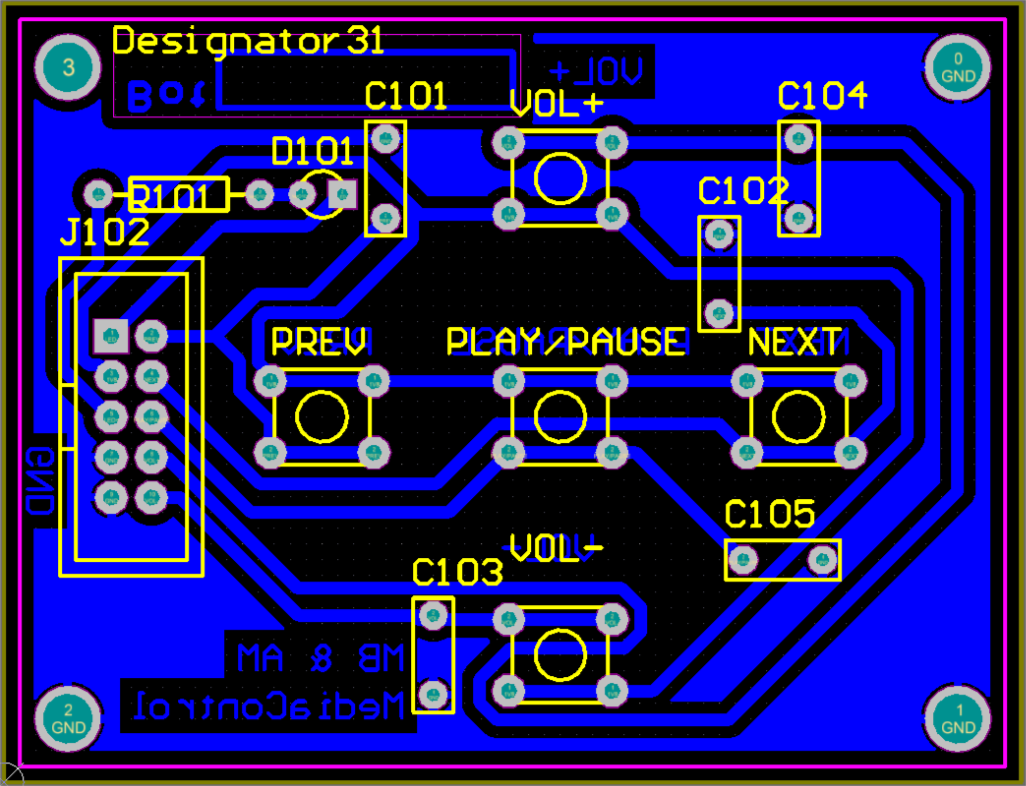
\includegraphics[width=1\textwidth]{schaltungen/front_pcb.png}
\end{figure} \\
Die Taster wurden in einem Kreuz aufgebaut, wobei an der linken oberen Ecke die Status-LED verbaut wurde.
\end{comment}







\null\newpage
\section{Tieftöner- und Hochtönerweiche}\label{kap:5.2}
\subsection{Allgemeines}\label{kap:5.2.1}
Für die Satellitenlautsprecher, welche aus einem Hochtöner und einem Tieftöner bestehen werden nun die Teilfrequenzbereiche Mitte und Hoch benötigt. Da es sich bei dem Satellitensystem um ein Paar an Boxen handelt und diese räumlichen weiter entfernt voneinander stehen, können nun Stereo-Effekte verwendet und mit dem reinen Stereo-Eingangssignal gearbeitet werden. Eine Aufteilung des Signals in Linke- und Rechte-Satellitenbox muss jedoch schon getroffen werden, um die Effekte richtig zu erhalten. Dafür wird einfach für die Linke-Satellitenbox, bestehend aus Hoch- und Tieftöner die entsprechenden Weichen verwendet und das Selbe für die Rechte-Box.

\subsection{Zielsetzung}\label{kap:5.2.2}
Das unberührte Eingangssignal soll so gefiltert werden, dass der Hochtöner nur Frequenzen über 1,5kHz und der Tieftöner Frequenzen bis 6kHz zum abstrahlen erhält. Dementsprechend sollen die Filter gewählt und designet werden.\\
Obwohl es den Mono-Bass gibt der die untersten Frequenzen (>20Hz) abzustrahlen hat, dürfen die Satelliten-Tieftöner im selbigen Bereich ebenfalls spielen. Somit wird die abstrahlende Fläche vergrößert und freiwerdende absolute Pegel höher. Bei dem Satelliten-Tieftöner wird jedoch ein Bandpass vorgesehen um bei möglichen Resonanzen mit dem Mono-Bass das Signal filtern zu können.\\
Dementsprechend sollen die Filter gewählt und designet werden.

\subsection{Filter}\label{kap:5.2.3}
Es wurden wie bereits in Kapitel \ref{kap:5.1} \enquote{Butterworth-Tiefpass-Filter 2. Ordnung} verwendet. Dieses mal ein Bandpass-Filter und ein Hochpass-Filter ebenfalls nach Butterworth. Dabei handelt es sich wieder um \enquote{Aktive-Filter} was bedeutet, dass OPV-Schaltungen verwendet wurden.\\
Das Bandpass-Filter(\ref{fig:abb5.2.3.1}) besteht aus drei Widerständen, zwei Kondensatoren und einem OPV dieser wird am Minus-Eingang angesteuert was zur folge hat, dass die Schaltung invertierend wirkt was aber keine Probleme aufbringt. Am Plus-Eingang des OPVs wird entweder Masse bei symmetrische Versorgungsspannung oder $\frac{Vcc}{2}$ bei asymmetrischer verwendet.
\begin{figure} [H]
	\centering
	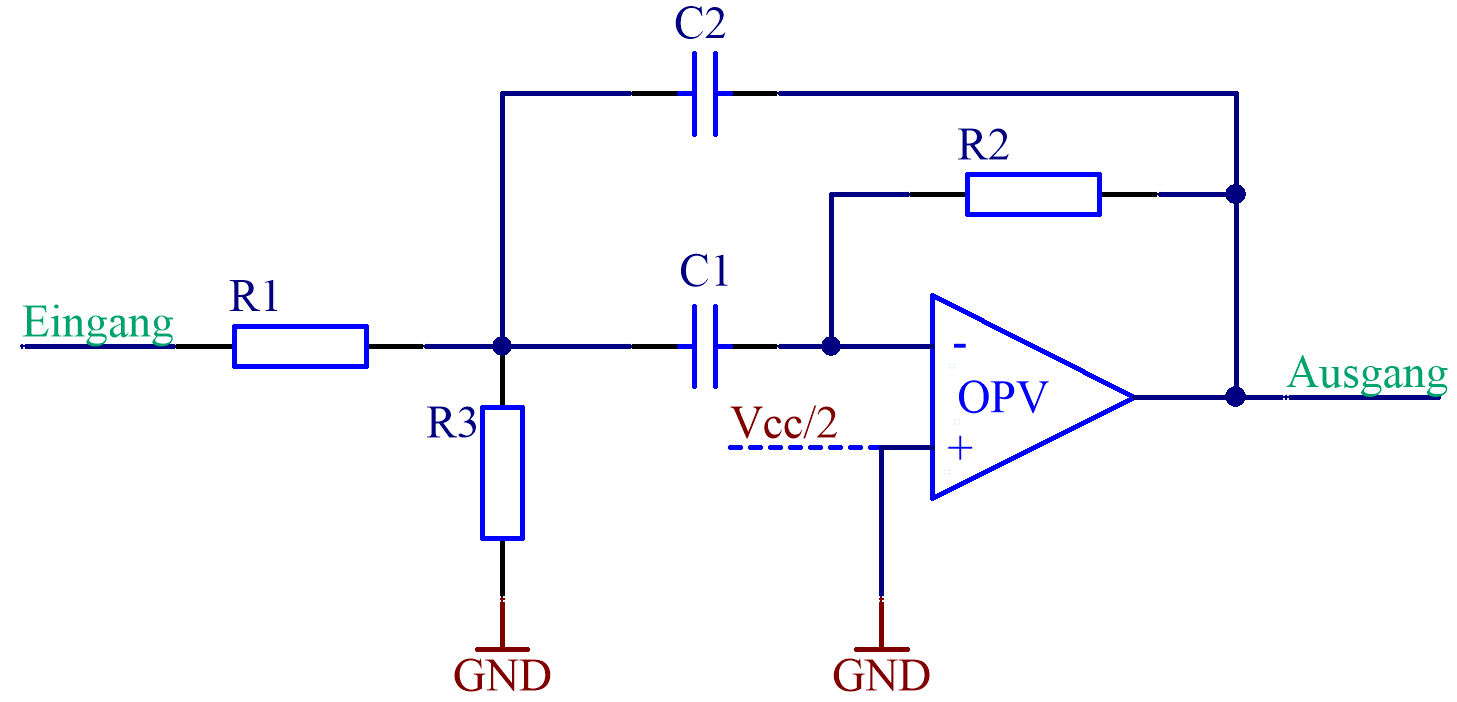
\includegraphics[width=1\textwidth]{img/Print4/BPFilter-Butterworth2Ordnung.PNG}
	\caption{Butterworth-Bandpass-Filter 2. Ordnung}
	\label {fig:abb5.2.3.1}
\end{figure}
Ähnliche Konstruktion hat der Hochpass(\ref{fig:abb5.2.3.2}). Dieser besteht aus drei Kondensatoren, zwei Widerständen und einem OPV.\\
\begin{figure} [H]
	\centering	
	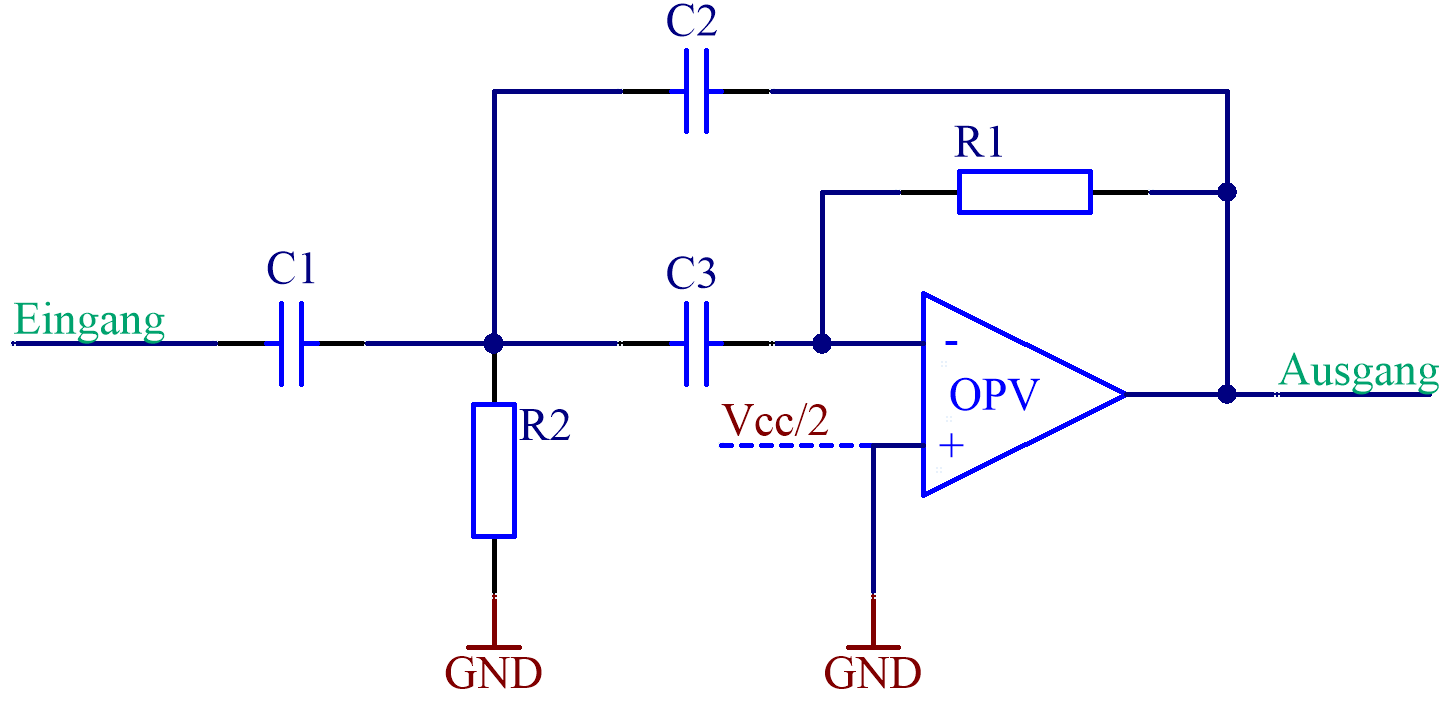
\includegraphics[width=1\textwidth]{img/Print4/HPFilter-Butterworth2Ordnung.PNG}
	\caption{Butterworth-Hochpass-Filter 2. Ordnung}
	\label {fig:abb5.2.3.2}
\end{figure}

\subsection{Schaltung}\label{kap:5.2.4}

Das Eingangssignal (Links, Rechts, Masse) wird an einer dreipoligen Stifleiste angeschlosssen (Abb. \ref{fig:abb5.2.4.1}). Zuerst gelangt Signal-Links und -Rechts an jeweils ein Potentiometer um den Pegel anpassen zu können, es bietet also eine Regelmöglichkeit. Es folgen die Filter. Hochpass für Links/Rechts und Tiefpass für Links/Rechts. Ein \enquote{Butterworth-Tiefpass-Filter 2. Ordnung} wurde bereits in dem Kapitel \ref{kap:5.1.4} erklärt. Das \enquote{Butterworth-Hochpass-Filter und -Bandpass-Filter 2. Ordnung} weist keine groben Unterschiede auf, der Unterschied liegt lediglich in der Bauteilaufteilung.\\
Nach den Filtern gelangen die getrennten Signale zu deren Ausgangspunkt. Es ist für jede Signalleitung eine zweipolige Stiftleist vorgesehen (Signal + Masse), da der darauffolgende Verstärker einen selbigen Eingang besitzt. Die Stiftleisten sind jedoch gruppiert nach Bandpass- und Hochpass-Ausgang.\\
\begin{figure} [H]
	\centering	
	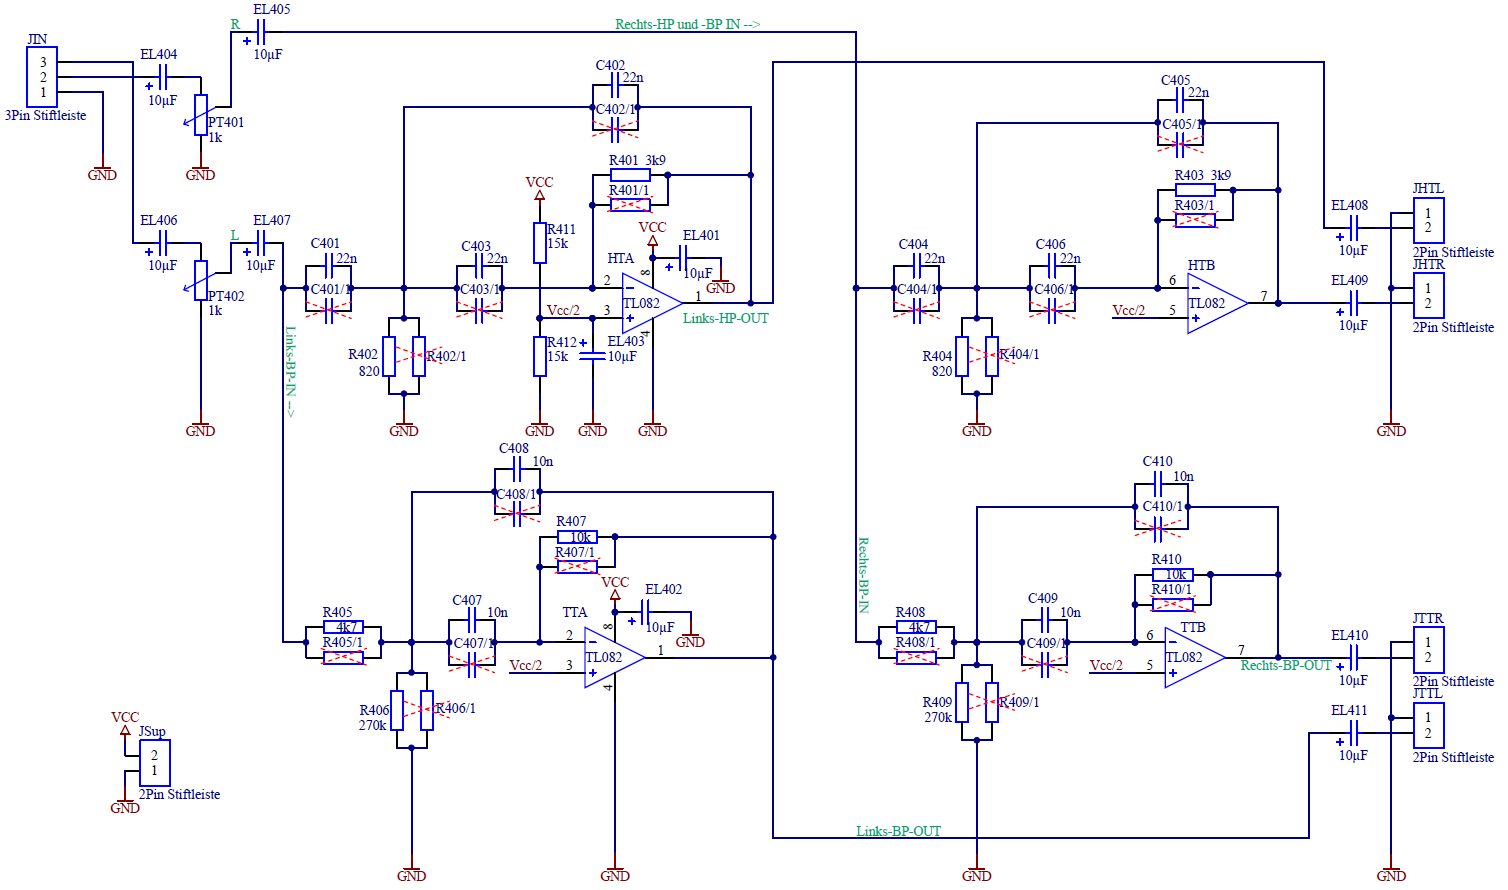
\includegraphics[width=1\textwidth]{img/Print4/4_TTuHTWeiche-Schematic.PNG}
	\caption{Butterworth-Bandpass-Filter 2. Ordnung}
	\label {fig:abb5.2.4.1}
\end{figure}
Eines der Bandpass-Filter. Gut sichtbar die doppelte, parallele Ausführung von Widerständen und Kondensatoren um krumme Werte auch erhalten zu können. Bedingt durch Parallel-Schaltung von Widerständen und Kondensatoren.\\ 
Der Eingang wurde gespiegelt um ein schöneres Bild zu erlangen. Die Spiegelung ist für das PCB-Layout nicht relevant!\\
Bedingt durch die Versorgungsspannung ist auch der Spannungsteiler für $\frac{Vcc}{2}$ am Plus-Eingang des OPVs implementiert.
\begin{figure} [H]
	\centering	
	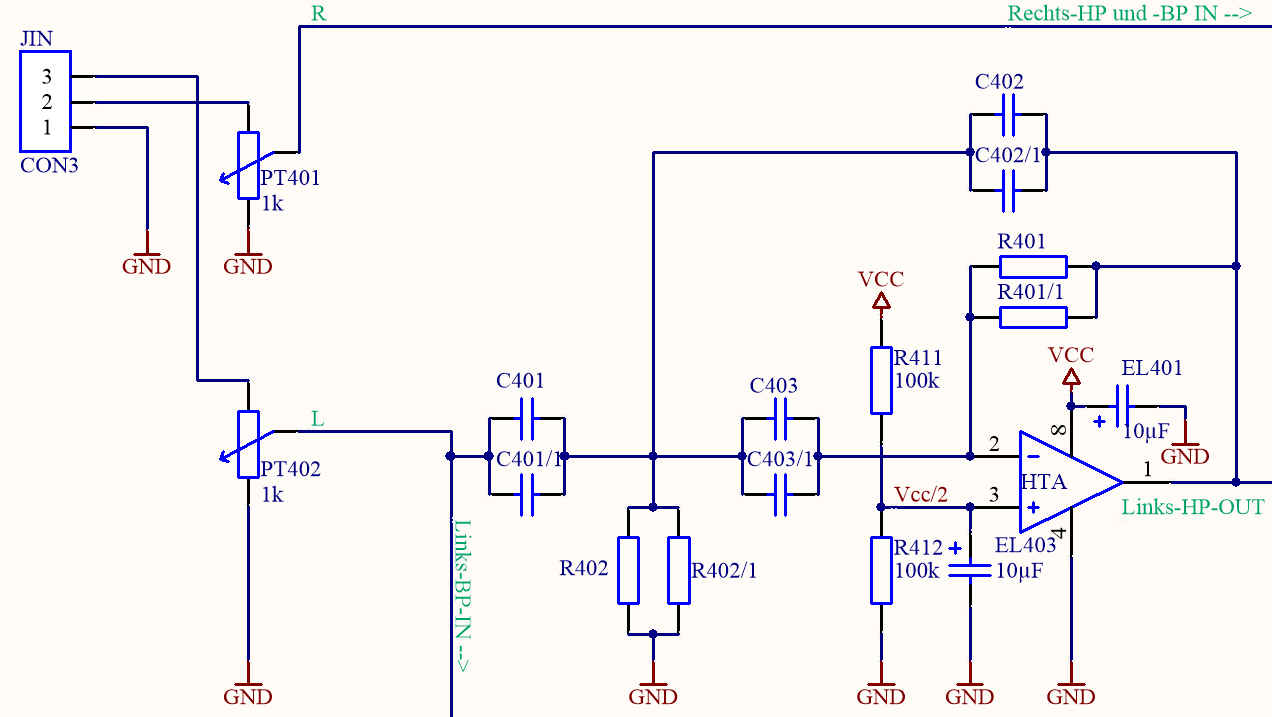
\includegraphics[width=1\textwidth]{img/Print4/4_TTuHTWeiche-LinksHP-Schematic.PNG}
	\caption{Butterworth-Bandpass-Filter 2. Ordnung - aus Abb.\ref{fig:abb5.2.4.1}}
	\label {fig:abb5.2.4.2}
\end{figure}
Am B-Teil des OPVs (erkennbar an der Beschriftung: TT\enquote{B}) ist keine Versorgung einzuzeichnen, da er mit dem A-Teil einen achtpinnigen IC mit zwei integrierten OPVs ergibt. Die zwei Teile sind über das IC-Gehäuse mit der gleichen Versorgungsspannung verbunden, deshalb ist das einmalige Kennzeichnen ausreichend.\\
\begin{figure} [H]
	\centering	
	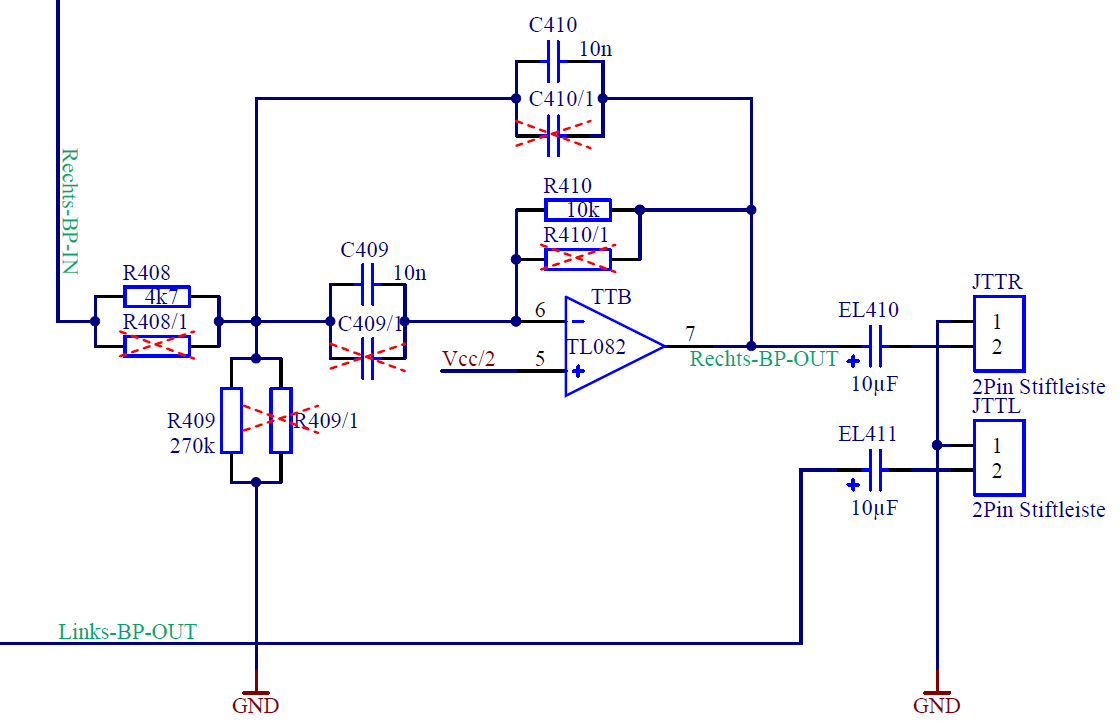
\includegraphics[width=1\textwidth]{img/Print4/4_TTuHTWeiche-RechtsBP-Schematic.PNG}
	\caption{Butterworth-Bandpass-Filter 2. Ordnung - aus Abb.\ref{fig:abb5.2.4.1}}
	\label {fig:abb5.2.4.3}
\end{figure}

\subsection{PCB}\label{kap:5.2.5}
Es wurden die grundlegenden Regeln zur Leiterplattenentflechtung angewandt (\ref{}). Bei dem Design (Abb. \ref{fig:abb5.2.5.1}) wurde auf hohe Variierbarkeit geachtet um auch zB. Kondensatoren mit unterschiedlichen Footprint verwenden zu können.\\
Es wurden wieder nahe an den IC's ELKOs in der Spannungsversorgungsleitung verbaut, um Störungen zu verhindern.

\begin{figure} [H]
	\centering	
	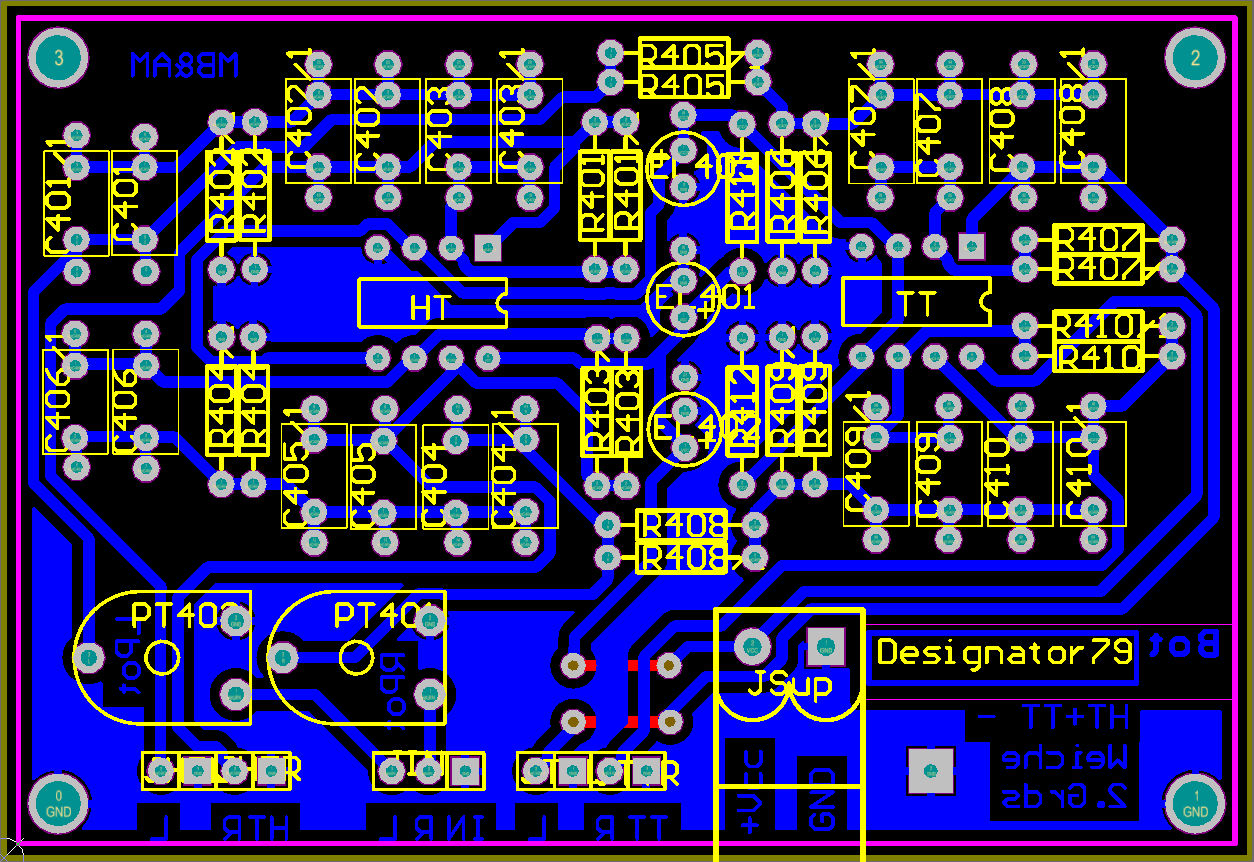
\includegraphics[width=1\textwidth]{img/Print4/4_TTuHTWeiche-PCB.PNG}
	\caption{Tieftöner- und Hochtönerweichen - PCB}
	\label {fig:abb5.2.5.1}
\end{figure}


\begin{comment}
%% Altium und Einstellungserklärung + Wichtige Layout-Faktoren
%Beim designen des Leiterplattenlayouts wurden die allgemeinen Altium-Einstellungen vorgenommen und auf die zu berücksichtigenden Layoutpunkte geachtet.
Beim \enquote{Layouten} der Schaltung mussten einige wichtige Faktoren berücksichtigt werden.\\
Wie da wären:\\
\begin{itemize}
	\item EMV-Technische-Faktoren, wie kurze Leiterbahnen
	\item Ausnützen der Printfläche
	\item Mehrfach-Footprints ermöglichen für verschiedene Bauteile
	\item Mechanische Aufhängebohrungen vorsehen
	\item Massefläche bei Möglichkeit vorsehen
\end{itemize}
Leiterplattenspezifische Einstellungen wurden aus den Kriterien der schuleigenen Leiterplattenfertigung übernommen. Zu diesen Einstellungen zählen:\\
\begin{itemize}
	\item Leiterbahnbreite
	\item Leiterbahnabstände untereinander
	\item Restring bei Bohrungen
	\item 
\end{itemize}

\subsection{Inbetriebnahme}
Bereits mit einer simplen Beschaltung kann das Modul in Betrieb genommen werden:
\begin{figure} [h]
	\centering
	\caption{Prinzipschaltung XS3868}
	\label {fig:abb2.3}
%%	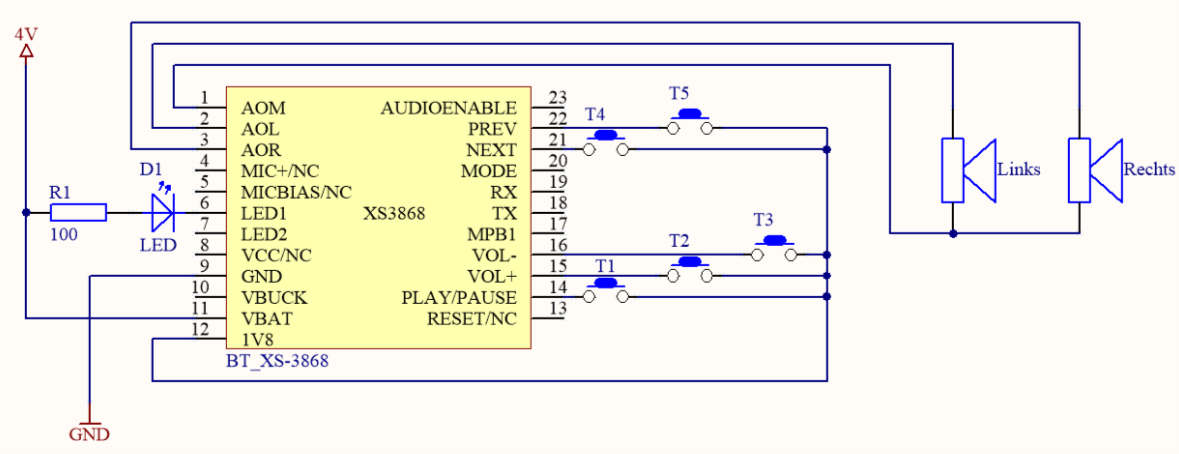
\includegraphics[width=1\textwidth]{schaltungen/XS3868_Prinzipschaltung.png}
\end{figure} \\
Mit dieser Schaltung (Abb. \ref {fig:abb2.3}) kann das Modul bereits ordnungsgemäß arbeiten.\\
Die Versorgungsspannung ist mit 4V etwas höher gewählt damit es nicht zu Ausfällen durch Spannungsschwankungen kommt. Das XS3868-Modul hat eine Stromaufnahme von ca. 30mA beim Starten, 10mA im Stand-By und bis zu 100mA wenn Musik abgespielt wird.\\ \\
Die Status-LED ist, wie in Abbildung \ref {fig:abb2.3} dargestellt, \enquote{Low-Aktiv}. Beim Starten des Moduls und während der Suche nach Geräten blinkt sie durchgehend, wobei sie bei einer bestehenden Verbindung nur die Hälfte der Zeit blinkt.\\ \\
Mit einfachem Betätigen eines Tasters wird die entsprechende Funktion vom Modul ausgeführt, jeweils mit einem Bestätigungston begleitet. Dieser Ton wird auch beim Starten des Moduls abgespielt.\\ \\
Statt die Lautsprecher direkt an das Modul anzuschließen, sollte allerdings noch ein Verstärker verbaut werden.
\newpage


\subsection{Verbindung mit dem Modul}
Wenn der OVC3860 eingeschaltet ist, sucht er andauernd nach BT-Geräten. Mit einem Smartphone findet man das Gerät und kann sich mit einem Standard-PIN-Code (\enquote{0000}) verbinden. Wenn bereits Lautsprecher angeschlossen sind, wird ein Ton abgespielt, der die Verbindung bestätigt. Außerdem hat die Status-LED nun ein anderes Blinkverhalten (Mehrmaliges Blinken mit längeren Pausen).\\ \\
Jetzt ist das Modul bereit Musik abzuspielen. Diese kann vom Smartphone oder vom Modul aus gesteuert werden. Die notwendigen Taster müssen allerdings schon in der Schaltung verbaut sein um die Bedienung der Musik zu ermöglichen.


\subsection{Zusatz-Leiterplatten}
\subsubsection{Allgemeines}
Als Entwicklungsprogramm für beide Leiterplatten wurde  \enquote{Altium Designer 13.3} verwendet. Die Schaltung wurde in diesem Programm gezeichnet, das Layout für die Leiterplatten angefertigt und entflechtet. Es wurden einseitige Platinen verwendet, da doppelseitige nicht notwendig waren.


\subsubsection{Adapter-Board}
Da das Modul in SMD-Bauform gefertigt ist, wurde ein Adapter-Board (Abb. \ref{fig:abb3.1}) vorgesehen um eine einfachere Handhabung mit dem Modul zu ermöglichen. Als Anschlussmöglichkeiten werden Stiftleisten verwendet.\\
Die Schaltung ist deshalb auch sehr simpel aufgebaut:
\begin{figure} [h]
	\centering
	\caption{Schaltung des Adapter-Boards}
	%%\label {fig:abb3.1}
%%	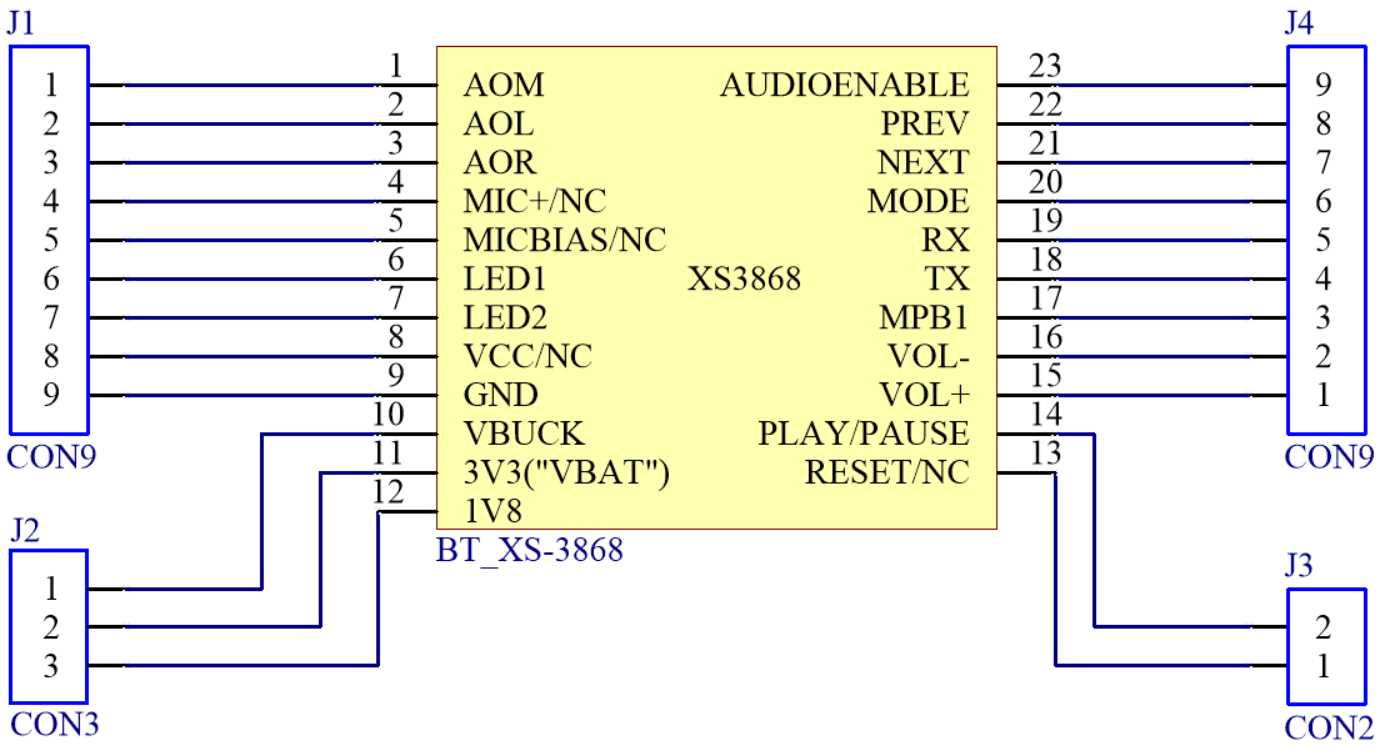
\includegraphics[width=1\textwidth]{schaltungen/adapter_sch.png}
\end{figure} \\
Jeder Pin bekommt auch auf dem Adapter einen eigenen Pin auf der Stiftleiste.
\newpage
Das PCB (Abb. \ref{fig:abb3.2}) ist, wie bereits erwähnt, einseitig aufgebaut:
\begin{figure} [h]
	\centering
	\caption{PCB des Adapter-Boards}
%%	\label {fig:abb3.2}
%%	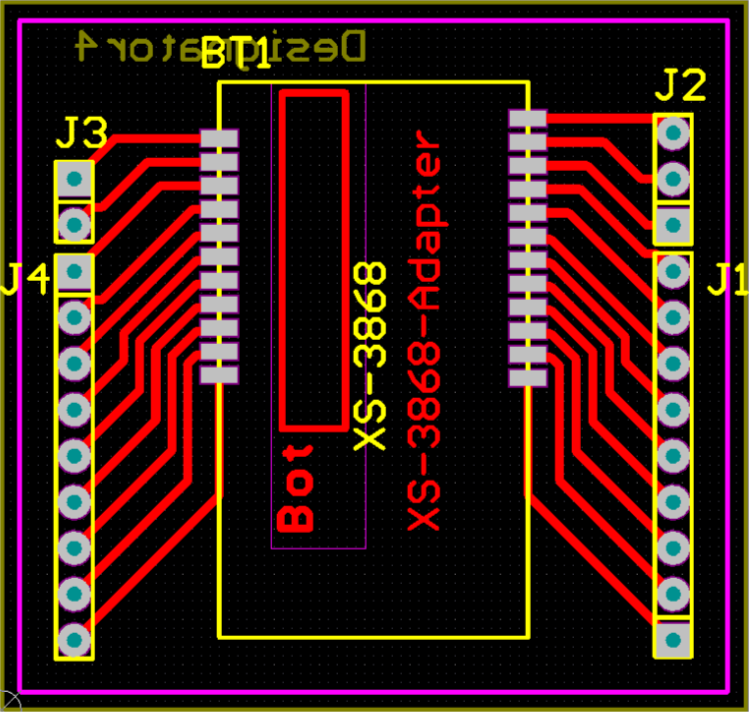
\includegraphics[width=1\textwidth]{schaltungen/adapter_pcb.png}
\end{figure} \\
Mit diesem PCB kann da BT-Modul nun besser getestet und auch weiterverwendet werden. Gemeinsam mit diesem Adapter kommt es auch auf das Hauptboard.
\newpage


\subsubsection{Hauptboard}
\minisec{Funktion}
Das Hauptboard wird hauptsächlich zur Versorgung des BT-Moduls, aber auch zur Weiterverarbeitung des Audio-Signals verwendet. Darüber hinaus ist eine Additionsschaltung vorgesehen, die das Signal des BT-Moduls mit einem zweiten, von einem Klinken-Eingang zugeführten, Signal vermischt. Die Lautstärke von diesem zweiten Audio-Signal kann über ein Stereo-Potentiometer geregelt werden. \\
Weiterhin sind die Pins zur Bedienung der Musik an einen 2x5-Wannenstecker herausgeführt. Zugang zur seriellen Schnittstelle wird auch ermöglicht.

\minisec{Schaltung}
Die Schaltung (Abb. \ref{fig:abb3.3}) des Hauptboards ist in mehrere Teile aufgeteilt und wird deshalb auch einzeln erklärt.
\begin{figure} [h]
	\centering
	\caption{Schaltung des Hauptboards (Versorgung + BT-Modul)}
%%	\label {fig:abb3.3}
%%	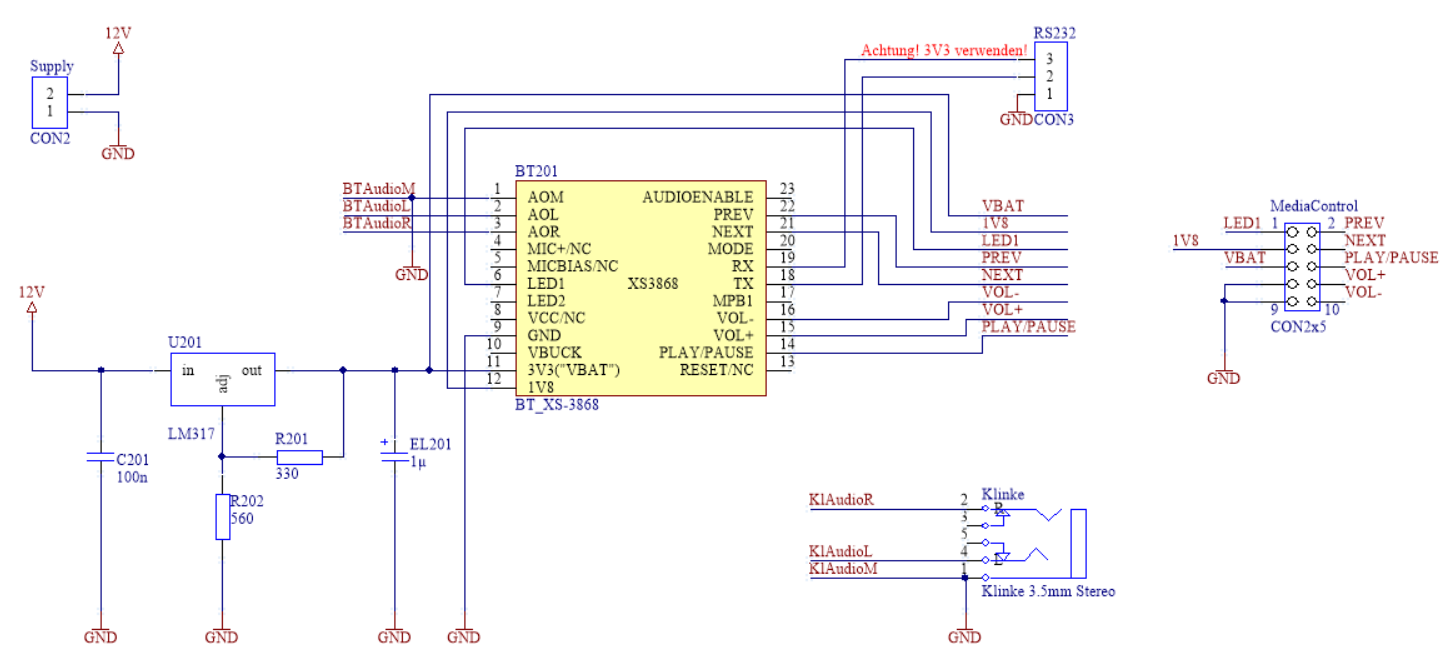
\includegraphics[width=1\textwidth]{schaltungen/hauptboard_sch1.png}
\end{figure} \\
In diesem Teil der Schaltung ist zu sehen: die Versorgungsbuchse, die Versorgungsschaltung für das BT-Modul, das BT-Modul mit herausgeführten Pins und die Klinken-Buchse.\\
Der Spannungsregler LM317 (Bezeichnung: U201) stellt eine Versorgungsspannung von 3,9V für das BT-Modul ein. Mit einer maximalen Stromaufnahme von 100mA ergibt sich folgende Verlustleistung:
\begin{equation}
	P_{max} = 7,9V * 100mA = 0,79W
\end{equation}
Deshalb wird auch kein Kühlkörper benötigt, es wird aber trotzdem eine Alu-Platte an den LM317 geschraubt um sicher zu gehen. \\
Ein eigener Stecker (Stiftleiste) für die Versorgung (12V) sowie die UART-Schnittstelle (RS232) sind auch vorgesehen. Der Wannenstecker (hier: \enquote{MediaControl}) ist mit allen wichtigen Pins des Moduls verbunden und verbindet eine Frontplatine mit dem Hauptboard. \\ \\
Die Klinkenbuchse wird in der folgenden Additionsschaltung(Abb. \ref {fig:abb3.4}) weiterverwendet:
\begin{figure} [h]
	\centering
	\caption{Schaltung des Hauptboards (Additionsschaltung)}
%%	\label {fig:abb3.4}
%%	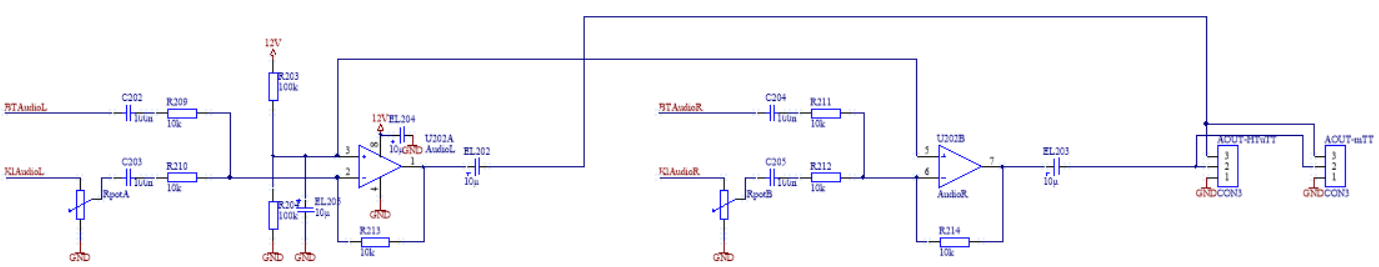
\includegraphics[width=1\textwidth]{schaltungen/hauptboard_sch2.png}
\end{figure} \\
Vergrößert:
\begin{figure} [h]
	\centering
	\caption{Schaltung des Hauptboards (linker Teil der Additionsschaltung)}
%%	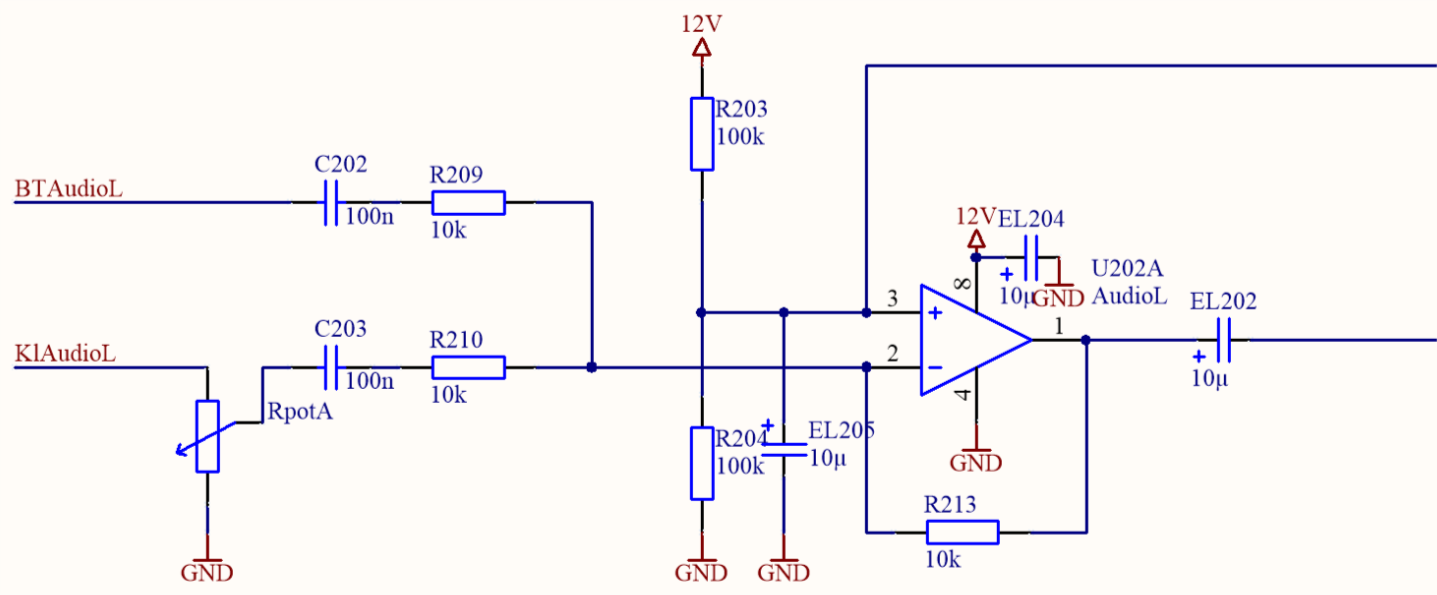
\includegraphics[width=1\textwidth]{schaltungen/hauptboard_sch2_zoom.png}
\end{figure} \\
Mithilfe dieser OPV-Schaltung werden die zwei Audio-Signale (ein Addierer pro Kanal) addiert. Das Signal vom Klinkeneingang kann zuvor noch mit einem Potentiometer abgeschwächt werden.\\
Der Arbeitspunkt bei 6V am Pin 3 wird benötigt um am Ausgang eine Spannung von $\pm$6V zu erreichen. Der OPV wird hier als invertierender Verstärker mit Verstärkung 1 aufgebaut, aber er addiert hier die zwei Signale zusammen auf ein Ausgangssignal.

\minisec{PCB}
Die Platine(Abb. \ref {fig:abb3.6}) für das Hauptboard sollte möglichst kompakt sein und alle Eingänge oder Bedienelemente auf einer Seite (hier rechts) haben. Das BT-Modul wird samt Adapter auf zwei Stiftleisten gesteckt. Darunter werden keine Bauteile verwendet, weil es sonst zu eng wäre. Des weiteren wären Bauteile unter dem Adapterprint während der Testphase unvorteilhaft, da diese schwerer zugänglich sind.
\begin{figure} [h]
	\centering
	\caption{PCB des Hauptboards}
%%	\label {fig:abb3.6}
	%%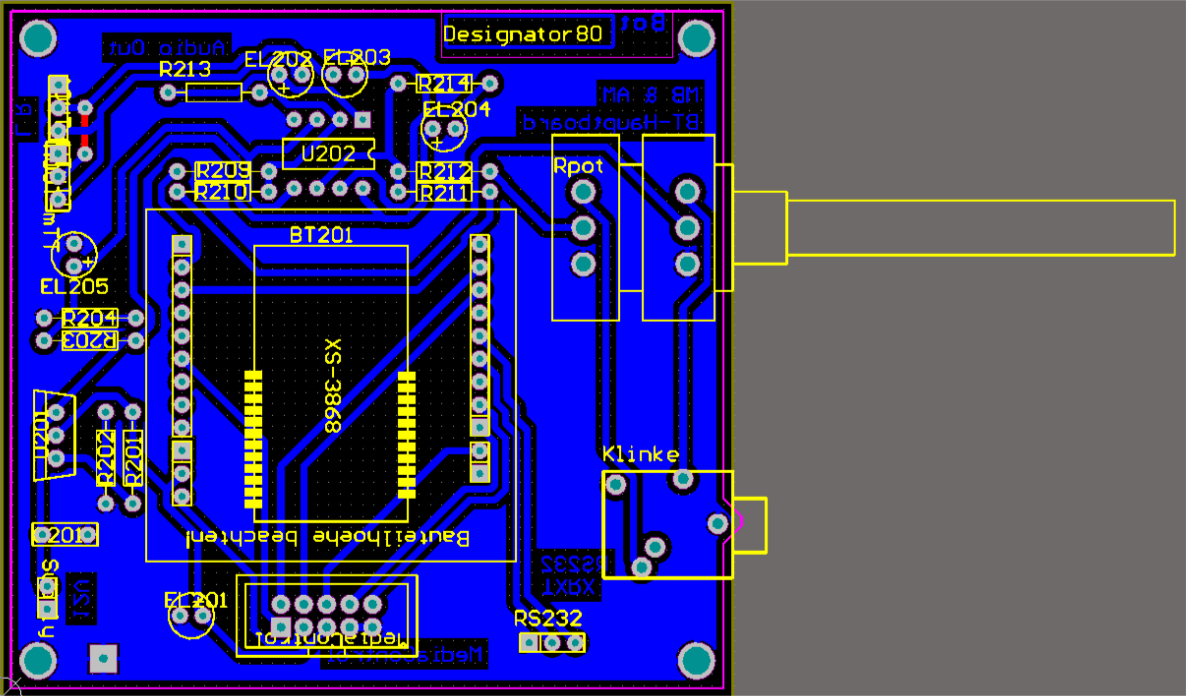
\includegraphics[width=1\textwidth]{schaltungen/hauptboard_pcb.png}
\end{figure}
\newpage


\subsubsection{Frontplatine}
\minisec{Funktion}
Diese Platine ist eigentlich eine Erweiterung des Hauptboards. Es wird mit dem Hauptboard über einen 2x5-Wannenstecker verbunden und auch versorgt. Sonst sind nur die Taster zur Bedienung des BT-Moduls, sowie die Status-LED verbaut.

\minisec{Schaltung}
Die Taster werden jeweils mithilfe eines Kondensators entprellt. Die Höhe der Taster reicht über die Kondensatoren hinaus um eine Bedienung zu ermöglichen. (Abb. \ref{fig:abb3.7})
\begin{figure} [h]
	\centering
	\caption{Schaltung der Frontplatine}
%%	\label {fig:abb3.7}
	%%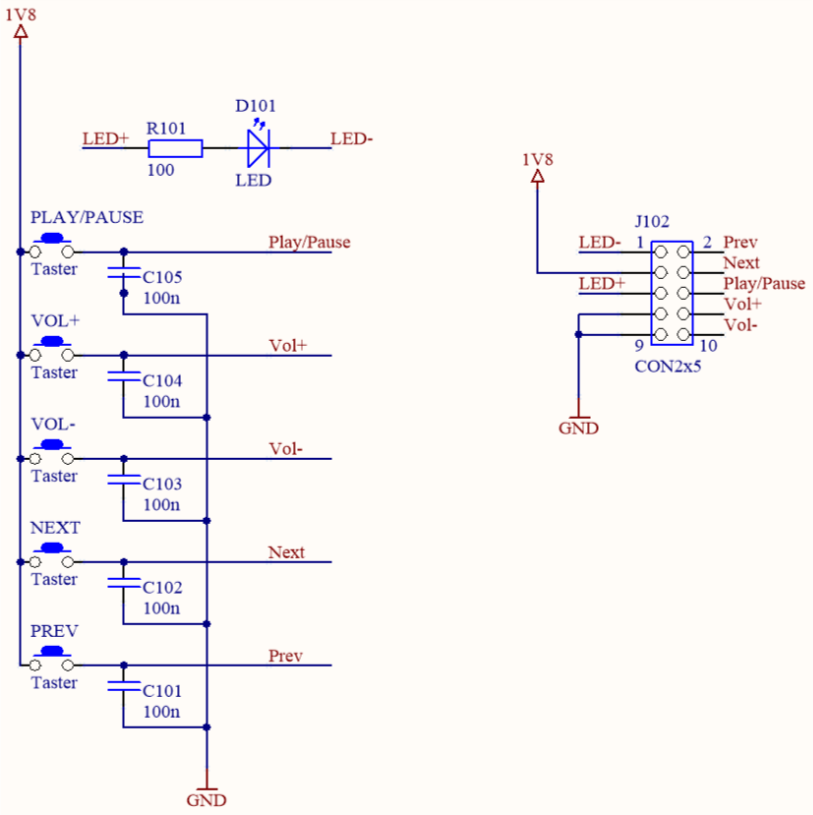
\includegraphics[width=0.7\textwidth]{schaltungen/front_sch.png}
\end{figure} \\
Jeder der Taster ist mit dem 1,8V-Pin des Moduls verbunden und geht dann weiter auf den entsprechenden Funktionspin. Die Bezeichnung \enquote{LED+} entspricht der Versorgungsspannung (\enquote{VBAT} = 3,9V) des Moduls. \enquote{LED-} ist mit dem Ansteuerungssignal am BT-Modul verbunden (Pin 6).

\minisec{PCB}
Das PCB (Abb. \ref {fig:abb3.8}) der Frontplatine soll ebenfalls so klein wie möglich aber von der Bedienung her sinnvoll aufgebaut sein.
\begin{figure} [h]
	\centering
	\caption{PCB der Frontplatine}
%%	\label {fig:abb3.8}
	%%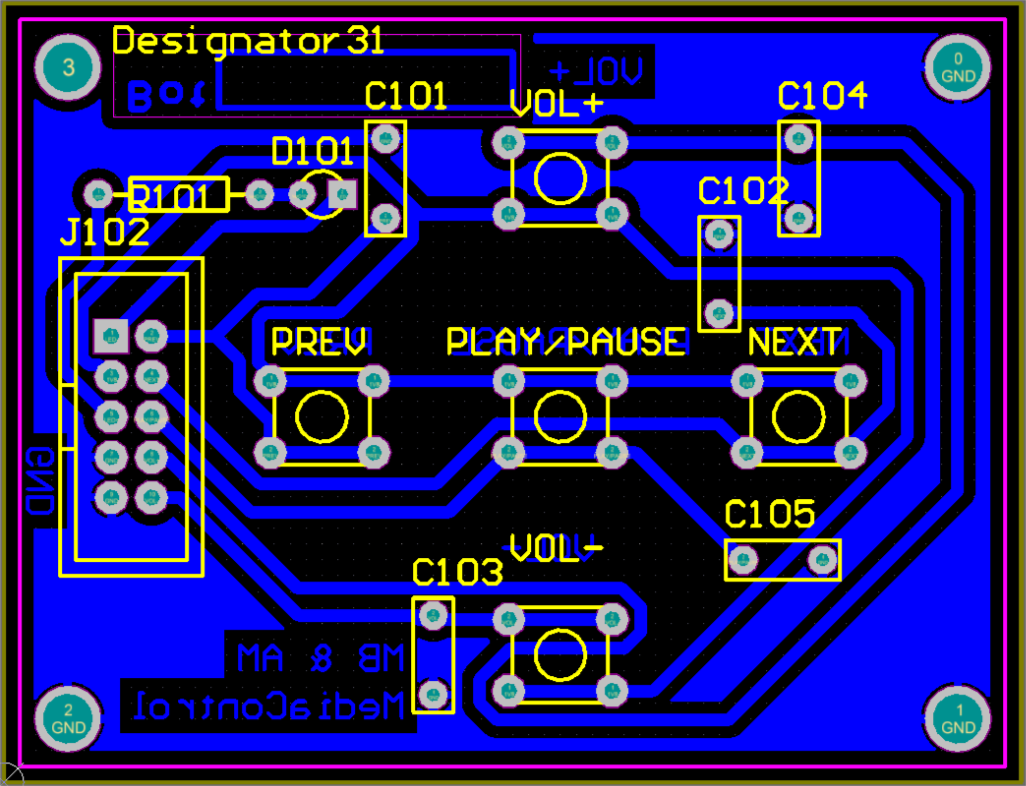
\includegraphics[width=1\textwidth]{schaltungen/front_pcb.png}
\end{figure} \\
Die Taster wurden in einem Kreuz aufgebaut, wobei an der linken oberen Ecke die Status-LED verbaut wurde.
\end{comment}







\newpage
\section{Tieftöner-Verstärker}\label{kap:5.3}
\subsection{Allgemeines}\label{kap:5.3.1}
Nach dem Filtern des Signals soll dieses vor dem Abstrahlen am Lautsprecher verstärkt werden. Es wurde eine analoge Verstärker-Schaltung verwendet, da diese einfacher und mit weniger Problemen realisiert werden hat können. Mit Hilfe bereits bekannter, bewährter Schaltungen konnte ein Layout für diese Schaltung designet werden. Ein wichtiger Baustein in dieser Schaltung ist der Verstärker \enquote{TDA2030}, wie in Kapitel \ref{kap:5.3.3} beschrieben.  Des weiteren wurden zwei Leistungstransistoren verbaut die höhere Ströme schalten können, falls der maximale Schaltstrom des TDA2030 erreicht wird.

\subsection{Zielsetzung}\label{kap:5.3.2}
Das Eingangssignal soll Verstärkt werden um am Ausgang der Schaltung höhere Spannungs-Amplituden und höheren Ströme aufzuweisen. Es soll nach diesem Schritt möglich sein den Tieftöner in einer der zwei Satellitenboxen mit ausreichend Signal zu versorgen, um einen Schalldruck von zumindest Zimmerlautstärke zu erhalten. 

\subsection{TDA2030}\label{kap:5.3.3}
Der TDA2030 ist ein für den Audio-Frequenzbereich optimierter OPV. Dieser kann symmetrisch sowie auch asymmetrisch versorgt werden. Eine typische Beschaltung ist im Datenblatt auch vorgegeben, welche auch verwendet wurde. Der TDA2030 besitzt ein Pentawatt-Gehäuse, welches deshalb auch eine Kühlfläche besitzt. Diese Kühlfläche hat das selbe Potential wie der mittlere Anschlusspin (Abb. \ref{5.3.3.1}).\\
Es wird auch für geringfügigen Betrieb ein Kühlkörper empfohlen!
\begin{figure} [ht]
	\centering
	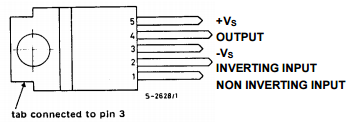
\includegraphics[width=1\textwidth]{img/Print5/TDA2030Pinning.PNG}
	\caption{TDA2030-Pinning}
	\label {fig:abb5.3.3.1}
\end{figure}
\subsubsection{Absolute Maximalwerte}
Diese Werte wurden zu aller erst mit den Bedingungen an der Schaltung verglichen, da sie ein sehr genaue, kurze Übersicht über den Baustein liefern.
\begin{figure} [ht]
	\centering
	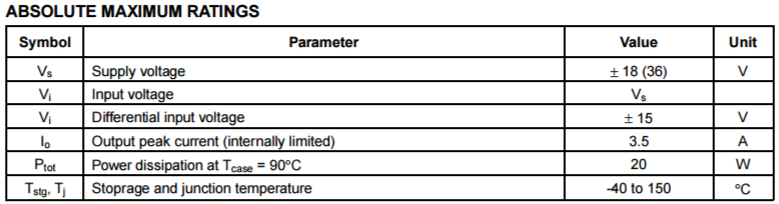
\includegraphics[width=1\textwidth]{img/Print5/TDA2030MaximumRatings.PNG}
	\caption{TDA2030-Pinning}
	\label {fig:abb5.3.3.2}
\end{figure}

\begin{comment}
\begin{figure} [ht]
	\centering	
	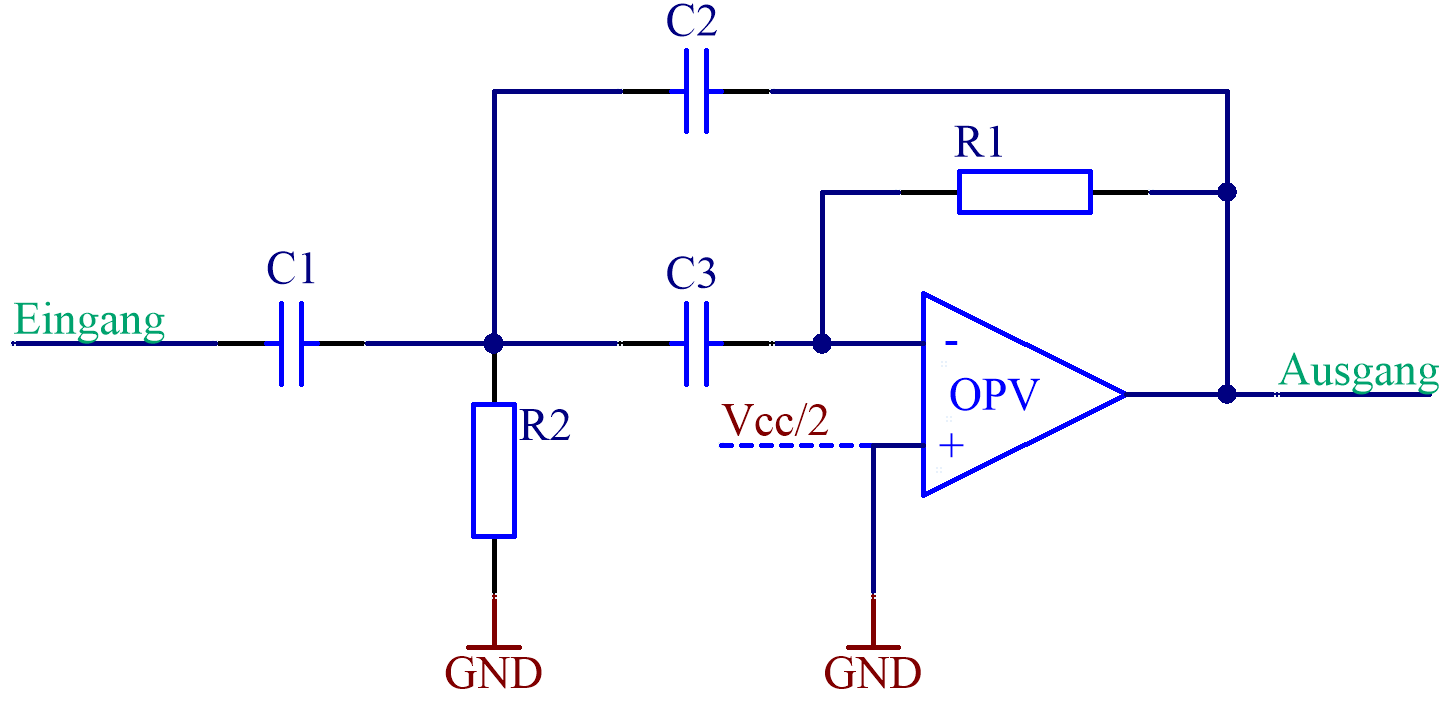
\includegraphics[width=1\textwidth]{img/Print4/HPFilter-Butterworth2Ordnung.PNG}
	\caption{Butterworth-Hochpass-Filter 2. Ordnung}
	\label {fig:abb5.2.3.2}
\end{figure}

\subsection{Schaltung}\label{kap:5.2.4}

Das Eingangssignal (Links, Rechts, Masse) wird an einer dreipoligen Stifleiste angeschlosssen (Abb. \ref{fig:abb5.2.4.1}). Zuerst gelangt Signal-Links und -Rechts an jeweils ein Potentiometer um den Pegel anpassen zu können, es bietet also eine Regelmöglichkeit. Es folgen die Filter. Hochpass für Links/Rechts und Tiefpass für Links/Rechts. Ein \enquote{Butterworth-Tiefpass-Filter 2. Ordnung} wurde bereits in dem Kapitel \ref{kap:5.1.4} erklärt. Das \enquote{Butterworth-Hochpass-Filter und -Bandpass-Filter 2. Ordnung} weist keine groben Unterschiede auf, der Unterschied liegt lediglich in der Bauteilaufteilung.\\
Nach den Filtern gelangen die getrennten Signale zu deren Ausgangspunkt. Es ist für jede Signalleitung eine zweipolige Stiftleist vorgesehen (Signal + Masse), da der darauffolgende Verstärker einen selbigen Eingang besitzt. Die Stiftleisten sind jedoch gruppiert nach Bandpass- und Hochpass-Ausgang.\\
\begin{figure} [ht]
	\centering	
	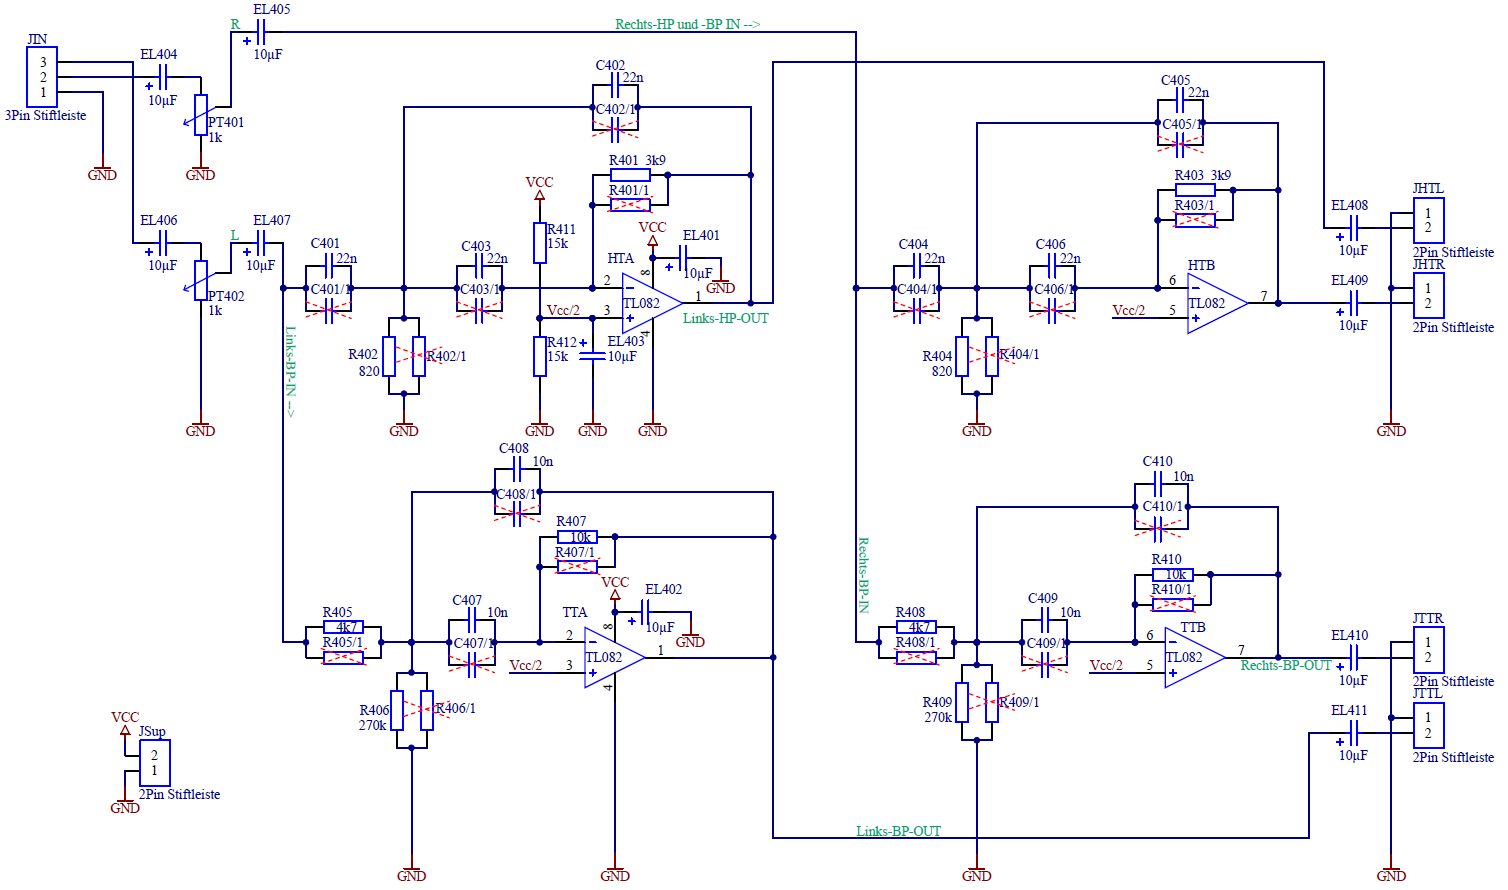
\includegraphics[width=1\textwidth]{img/Print4/4_TTuHTWeiche-Schematic.PNG}
	\caption{Butterworth-Bandpass-Filter 2. Ordnung}
	\label {fig:abb5.2.4.1}
\end{figure}\\
Eines der Bandpass-Filter. Gut sichtbar die doppelte, parallele Ausführung von Widerständen und Kondensatoren um krumme Werte auch erhalten zu können. Bedingt durch Parallel-Schaltung von Widerständen und Kondensatoren.\\ 
Der Eingang wurde gespiegelt um ein schöneres Bild zu erlangen. Die Spiegelung ist für das PCB-Layout nicht relevant!\\
Bedingt durch die Versorgungsspannung ist auch der Spannungsteiler für $\frac{Vcc}{2}$ am Plus-Eingang des OPVs implementiert.
\begin{figure} [ht]
	\centering	
	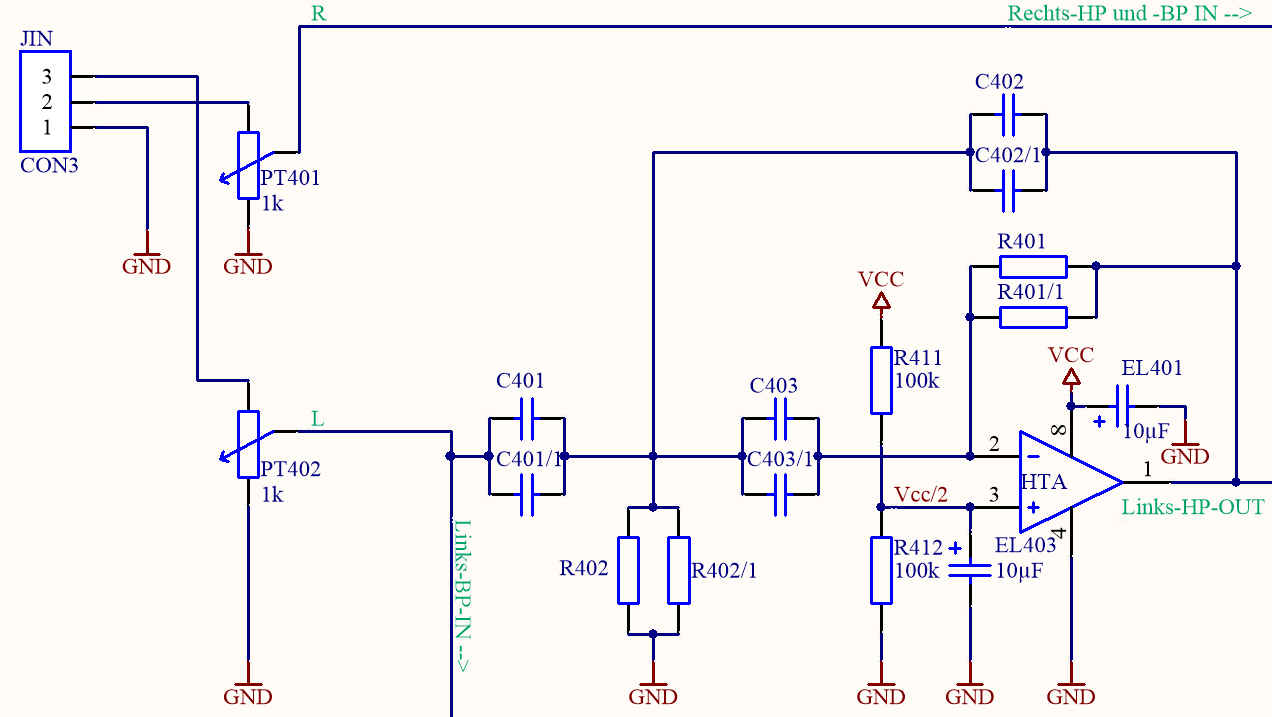
\includegraphics[width=1\textwidth]{img/Print4/4_TTuHTWeiche-LinksHP-Schematic.PNG}
	\caption{Butterworth-Bandpass-Filter 2. Ordnung - aus Abb.\ref{fig:abb5.2.4.1}}
	\label {fig:abb5.2.4.2}
\end{figure}\\
Am B-Teil des OPVs (erkennbar an der Beschriftung: TT\enquote{B}) ist keine Versorgung einzuzeichnen, da er mit dem A-Teil einen achtpinnigen IC mit zwei integrierten OPVs ergibt. Die zwei Teile sind über das IC-Gehäuse mit der gleichen Versorgungsspannung verbunden, deshalb ist das einmalige Kennzeichnen ausreichend.\\
\begin{figure} [ht]
	\centering	
	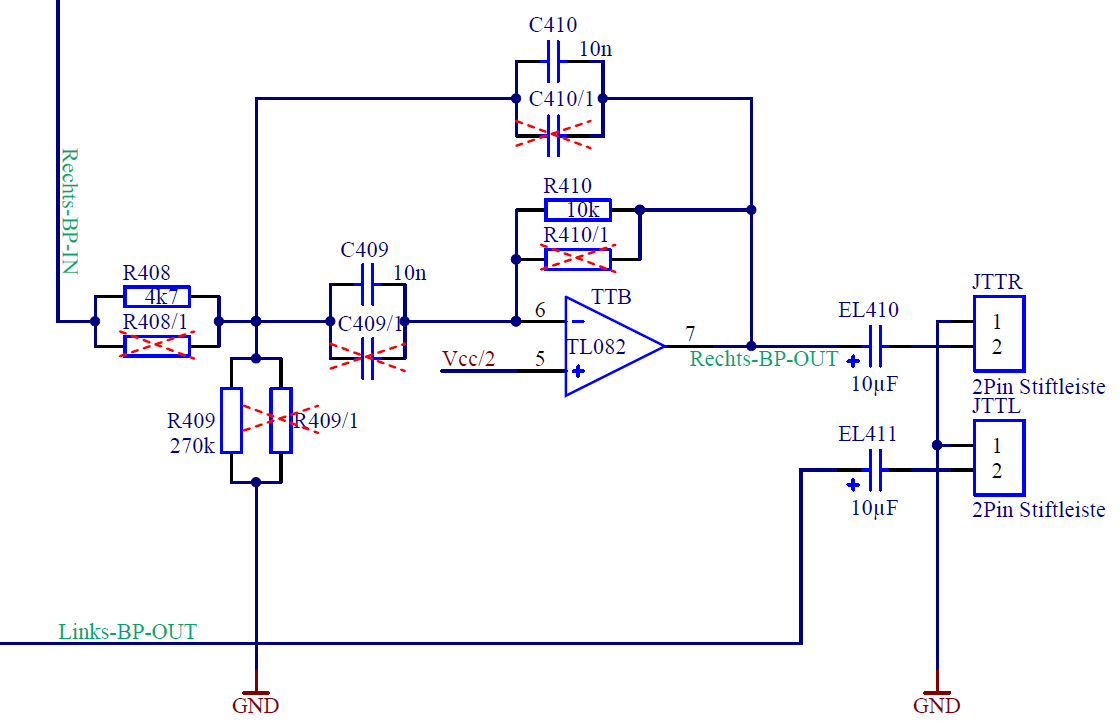
\includegraphics[width=1\textwidth]{img/Print4/4_TTuHTWeiche-RechtsBP-Schematic.PNG}
	\caption{Butterworth-Bandpass-Filter 2. Ordnung - aus Abb.\ref{fig:abb5.2.4.1}}
	\label {fig:abb5.2.4.3}
\end{figure}

\subsection{PCB}\label{kap:5.2.5}
Es wurden die grundlegenden Regeln zur Leiterplattenentflechtung angewandt (\ref{}). Bei dem Design (Abb. \ref{fig:abb5.2.5.1}) wurde auf hohe Variierbarkeit geachtet um auch zB. Kondensatoren mit unterschiedlichen Footprint verwenden zu können.\\
Es wurden wieder nahe an den IC's ELKOs in der Spannungsversorgungsleitung verbaut, um Störungen zu verhindern.

\begin{figure} [ht]
	\centering	
	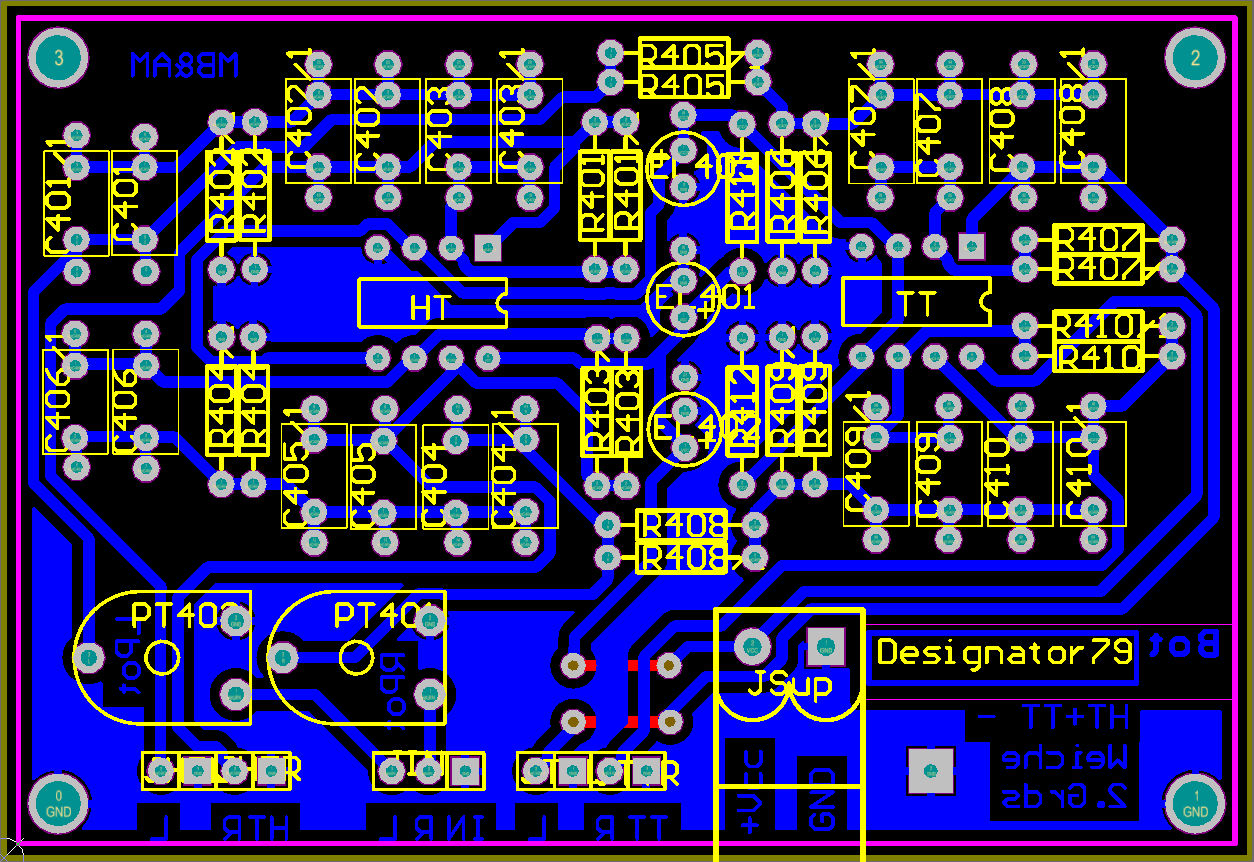
\includegraphics[width=1\textwidth]{img/Print4/4_TTuHTWeiche-PCB.PNG}
	\caption{Tieftöner- und Hochtönerweichen - PCB}
	\label {fig:abb5.2.5.1}
\end{figure}


\begin{comment}
%% Altium und Einstellungserklärung + Wichtige Layout-Faktoren
%Beim designen des Leiterplattenlayouts wurden die allgemeinen Altium-Einstellungen vorgenommen und auf die zu berücksichtigenden Layoutpunkte geachtet.
Beim \enquote{Layouten} der Schaltung mussten einige wichtige Faktoren berücksichtigt werden.\\
Wie da wären:\\
\begin{itemize}
	\item EMV-Technische-Faktoren, wie kurze Leiterbahnen
	\item Ausnützen der Printfläche
	\item Mehrfach-Footprints ermöglichen für verschiedene Bauteile
	\item Mechanische Aufhängebohrungen vorsehen
	\item Massefläche bei Möglichkeit vorsehen
\end{itemize}
Leiterplattenspezifische Einstellungen wurden aus den Kriterien der schuleigenen Leiterplattenfertigung übernommen. Zu diesen Einstellungen zählen:\\
\begin{itemize}
	\item Leiterbahnbreite
	\item Leiterbahnabstände untereinander
	\item Restring bei Bohrungen
	\item 
\end{itemize}
\end{comment}








%% ANHANG ==============================================%%
\appendix

%% abkürzungsverzeichnis ===============================%%
%% start of file abkuerzungen.tex

% Abkuerzungsverzeichnis
\addchap{
	\iflanguage{english}{Acronyms}{Abkürzungsverzeichnis}}
\begin{acronym}[ACRONYM]
\acro{tikz}[TikZ]{\TikZ{} ist kein Zeichenprogramm}
\acro{spi}[SPI]{Serial Peripheral Interface}
\end{acronym}\newpage

%% end of file abkuerzungen.tex
%%======================================================%%

%% abbildungsverzeichnis ===============================%%
\setcounter{lofdepth}{2}
\dipalistoffigures
%%======================================================%%

%% tabellenverzeichnis =================================%%
\setcounter{lotdepth}{2}
\dipalistoftables
%%======================================================%%

%% danksagungen=========================================%%
\newpage
\begin{acknowledgements}
    Wir bedanken uns bei
    \subparagraph{Prof. Dipl.-Ing. Dr. Herbert Wagner} für die tatkräftige Unterstützung und das ermöglichen eines einwandfreien Arbeitens an unserer Diplomarbeit und dem Projekt.
    %\subparagraph{FL Ing. DEFG} für ...
\end{acknowledgements}

%%======================================================%%

%% literaturverzeichnis ================================%%
\newpage
\begin{literature}
% The TeXbook by D. E. Knuth
\bibitem[1]{TeXbooooook}{\textbf{Donald~E.~Knuth:} \emph{The \TeX{}book}. 1986, {\scshape Addison--Wesley} Verlag,\\ ISBN-13: 978-0-201-13447-6}
\bibitem[2]{TDA2030Amp}{\textbf{Herbert Sax:} SGS-Ates TDA2030 , {\scshape SGS-Ates} Verlag,\\ ISBN-13: -}

\end{literature}
 
%%======================================================%%

%% betreuungsprotokolle ================================%%
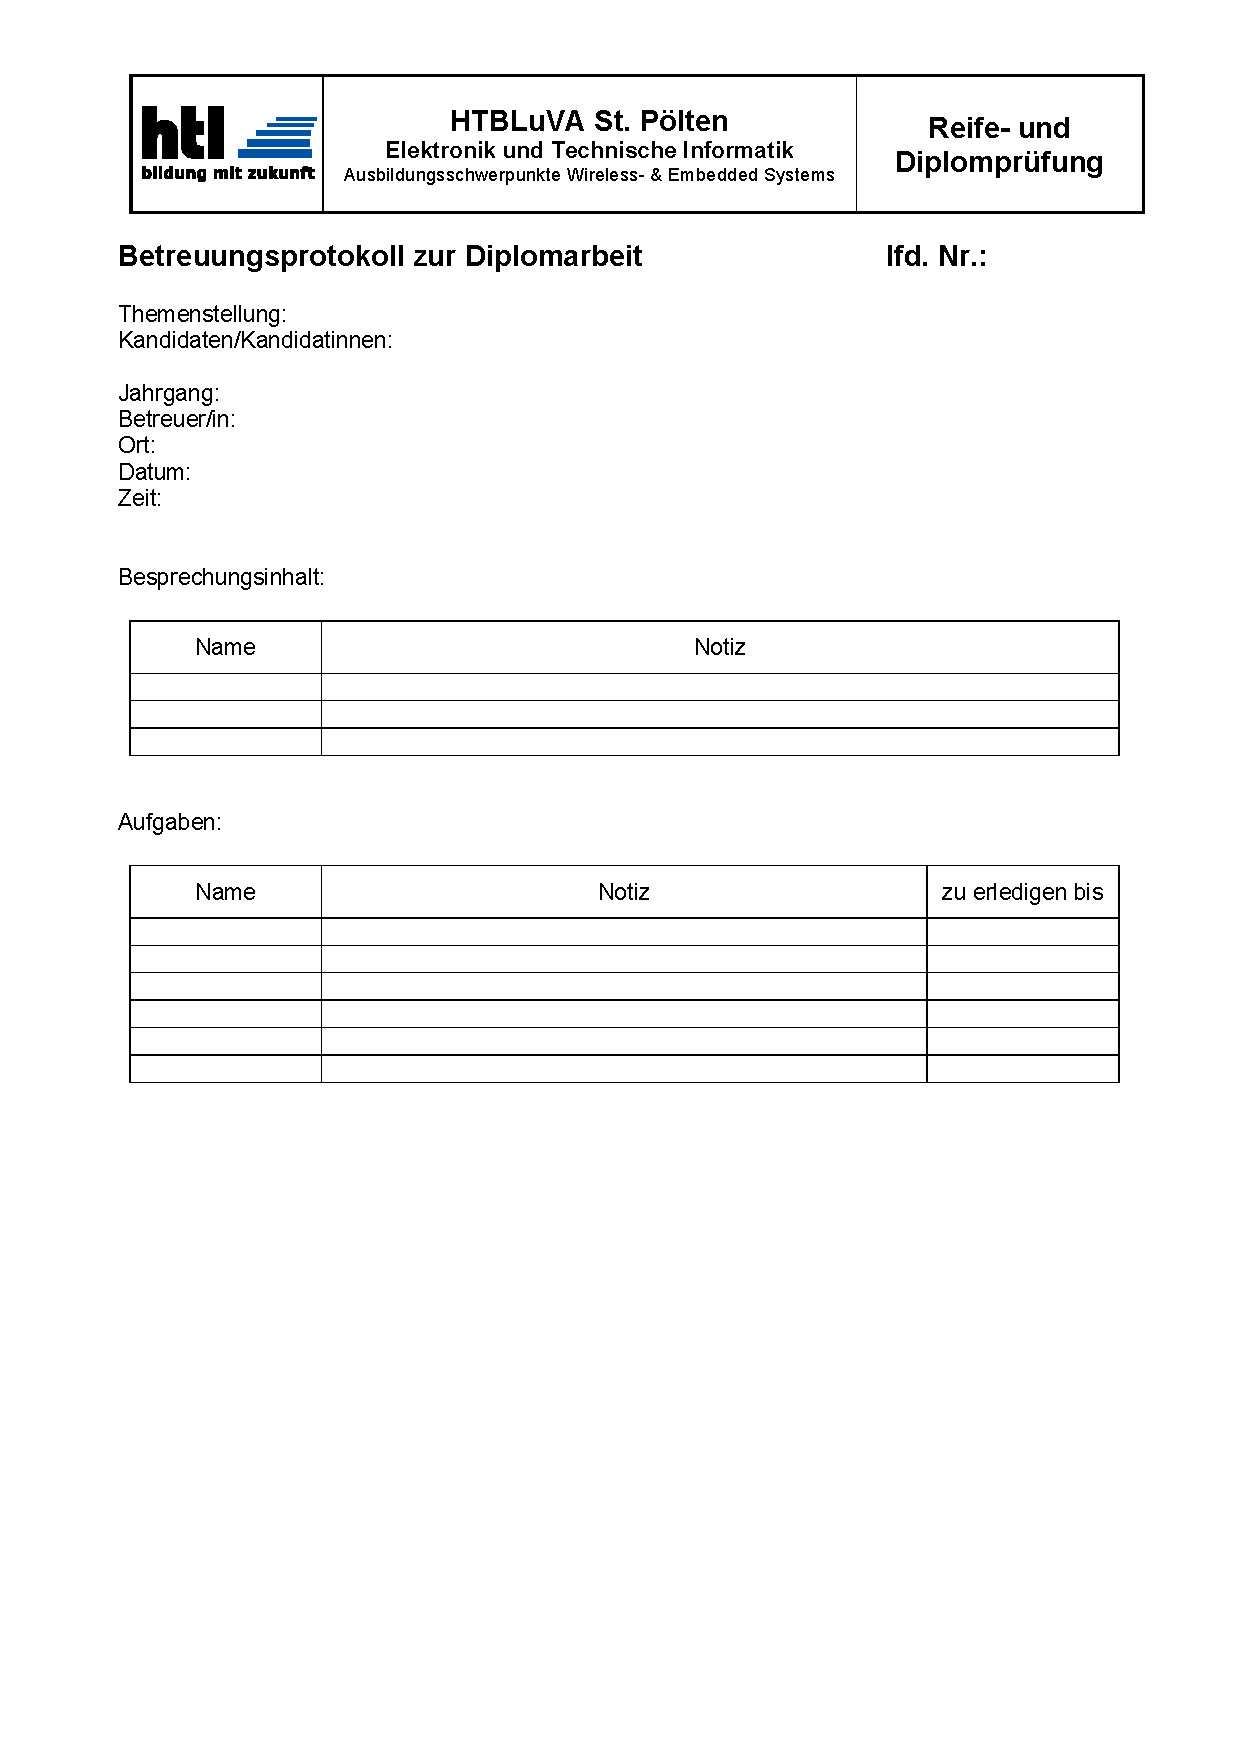
\includepdf[pages=-]{form/betreuungsprotokoll_1.pdf}
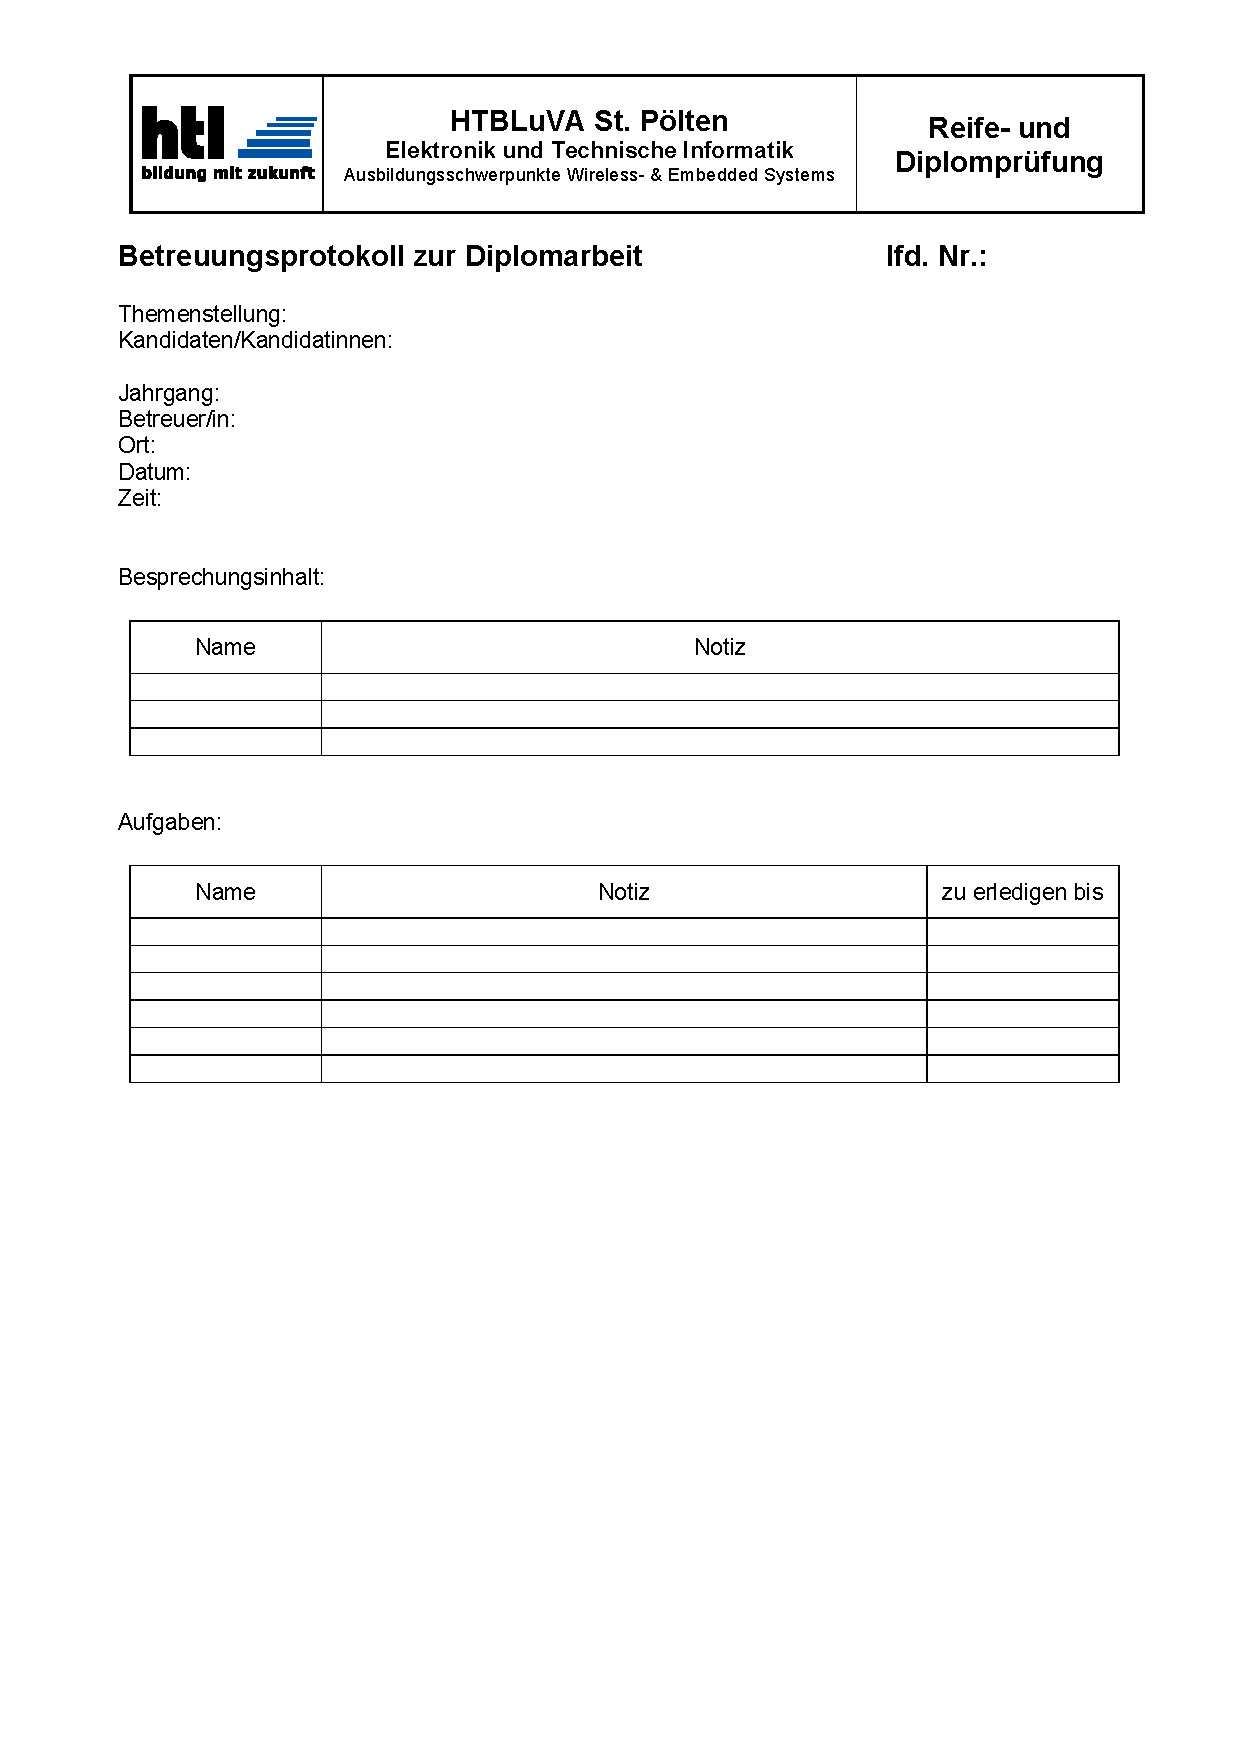
\includepdf[pages=-]{form/betreuungsprotokoll_2.pdf}
%% =====================================================%%

\end{document}
